%\section{Systematics Uncertainties on the Background Prediction}
%\label{sec:systematics}

[DESCRIBE HERE ONE BY ONE THE UNCERTAINTIES THAT ARE PRESENT IN THE SPREADSHHET
FROM WHICH WE CALCULATE THE TOTAL UNCERTAINTY. WE KNOW HOW TO DO THIS
AND
WE HAVE THE TECHNOLOGY FROM THE 7 TEV ANALYSIS TO PROPAGATE ALL
UNCERTAINTIES
CORRECTLY THROUGH.  WE WILL DO IT ONCE WE HAVE SETTLED ON THE
INDIVIDUAL PIECES WHICH ARE STILL IN FLUX]

In this Section we discuss the systematic uncertainty on the BG
prediction.  This prediction is assembled from the event
counts in the peak region of the transverse mass distribution as
well as Monte Carlo 
with a number of correction factors, as described previously.
The
final uncertainty on the prediction is built up from the uncertainties in these
individual 
components. 
The calculation is done for each signal
region,
for electrons and muons separately.

The choice to normalizing to the peak region of $M_T$ has the
advantage that some uncertainties, e.g., luminosity, cancel.
It does however introduce complications because it couples
some of the uncertainties in non-trivial ways.  For example, 
the primary effect of an uncertainty on the rare MC cross-section
is to introduce an uncertainty in the rare MC background estimate
which comes entirely from MC.   But this uncertainty also affects,
for example,
the $t\bar{t} \to$ dilepton BG estimate because it changes the 
$t\bar{t}$ normalization to the peak region (because some of the 
events in the peak region are from rare processes).  These effects
are carefully accounted for.  The contribution to the overall
uncertainty from each BG source is tabulated in
Section~\ref{sec:bgunc-bottomline}.
First, however, we discuss the uncertainties one-by-one and we comment 
on their impact on the overall result, at least to first order.
Second order effects, such as the one described, are also included.

\subsection{Statistical uncertainties on the event counts in the $M_T$
peak regions}
These vary between XX and XX \%, depending on the signal region
(different
signal regions have different \met\ requirements, thus they also have
different $M_T$ regions used as control.
Since 
the major BG, eg, $t\bar{t}$ are normalized to the peak regions, this 
fractional uncertainty is pretty much carried through all the way to
the end.  There is also an uncertainty from the finite MC event counts
in the $M_T$ peak regions.  This is also included, but it is smaller.

\subsection{Uncertainty from the choice of $M_T$ peak region}
IN 7 TEV DATA WE HAD SOME SHAPE DIFFERENCES IN THE MTRANS REGION THAT 
LED US TO CONSERVATIVELY INCLUDE THIS UNCERTAINTY.  WE NEED TO LOOK
INTO THIS AGAIN

\subsection{Uncertainty on the Wjets cross-section and the rare MC cross-sections}
These are taken as 50\%, uncorrelated.  
The primary effect is to introduce a 50\%
uncertainty
on the $W +$ jets and rare BG 
background predictions, respectively.  However they also
have an effect on the other BGs via the $M_T$ peak normalization
in a way that tends to reduce the uncertainty.  This is easy
to understand: if the $W$ cross-section is increased by 50\%, then
the $W$ background goes up.  But the number of $M_T$ peak events 
attributed to $t\bar{t}$ goes down, and since the $t\bar{t}$ BG is
scaled to the number of $t\bar{t}$ events in the peak, the $t\bar{t}$ 
BG goes down.  

\subsection{Scale factors for the tail-to-peak ratios for lepton +
  jets top and W events}
These tail-to-peak ratios are described in Section~\ref{sec:ttp}.
They are studied in CR1 and CR2.  The studies are described
in Sections~\ref{sec:cr1} and~\ref{sec:cr2}), respectively, where 
we also give the uncertainty on the scale factors.

\subsection{Uncertainty on extra jet radiation for dilepton
  background}
As discussed in Section~\ref{sec:jetmultiplicity}, the 
jet distribution in
$t\bar{t} \to$
dilepton MC is rescaled by the factors $K_3$ and $K_4$ to make 
it agree with the data.  The XX\% uncertainties on $K_3$ and $K_4$
comes from data/MC statistics.  This  
result directly in a XX\% uncertainty on the dilepton BG, which is by far 
the most important one.


\subsection{Uncertainty on the \ttll\ Acceptance}

The \ttbar\ background prediction is obtained from MC, with corrections
derived from control samples in data. The uncertainty associated with
the theoretical modeling of the \ttbar\ production and decay is
estimated by comparing the background predictions obtained using 
alternative MC samples. It should be noted that the full analysis is
performed with the alternative samples under consideration, 
including the derivation of the various data-to-MC scale factors. 
The variations considered are

\begin{itemize}
\item Top mass: The alternative values for the top mass differ
  from the central value by $5~\GeV$: $m_{\mathrm{top}} = 178.5~\GeV$ and $m_{\mathrm{top}}
  = 166.5~\GeV$.
\item Jet-parton matching scale: This corresponds to variations in the
  scale at which the Matrix Element partons from Madgraph are matched
  to Parton Shower partons from Pythia. The nominal value is
  $x_q>20~\GeV$. The alternative values used are $x_q>10~\GeV$ and
  $x_q>40~\GeV$.
\item Renormalization and factorization scale: The alternative samples
  correspond to variations in the scale $\times 2$ and $\times 0.5$. The nominal
  value for the scale used is $Q^2 = m_{\mathrm{top}}^2 +
  \sum_{\mathrm{jets}} \pt^2$.
\item Alternative generators: Samples produced with different
  generators include MC@NLO and Powheg (NLO generators) and
  Pythia (LO). It may also be noted that MC@NLO uses Herwig6 for the 
  hadronisation, while POWHEG uses Pythia6.
\item Modeling of taus: The alternative sample does not include
  Tauola and is otherwise identical to the Powheg sample.
  This effect was studied earlier using 7~TeV samples and found to be negligible.
\item The PDF uncertainty is estimated following the PDF4LHC
  recommendations[CITE]. The events are reweighted using alternative
  PDF sets for CT10 and MSTW2008 and the uncertainties for each are derived using the
  alternative eigenvector variations and the ``master equation''. In
  addition, the NNPDF2.1 set with 100 replicas. The central value is
  determined from the mean and the uncertainty is derived from the
  $1\sigma$ range. The overall uncertainty is derived from the envelope of the
  alternative predictions and their uncertainties.
  This effect was studied earlier using 7~TeV samples and found to be negligible.
  \end{itemize}


\begin{figure}[hbt]
  \begin{center}
	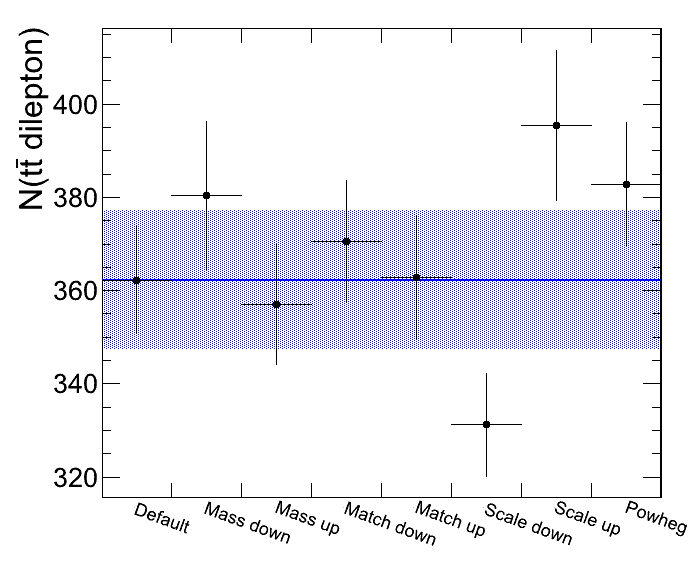
\includegraphics[width=0.8\linewidth]{plots/n_dl_syst_comp.png}
	\caption{
	  \label{fig:ttllsyst}%\protect 
          Comparison of the \ttll\ central prediction with those using
          alternative MC samples. The blue band corresponds to the
          total statistical error for all data and MC samples. The
          alternative sample predictions are indicated by the
          datapoints. The uncertainties on the alternative predictions
          correspond to the uncorrelated statistical uncertainty from
          the size of the alternative sample only.
        [TO BE UPDATED WITH THE LATEST SELECTION AND SFS]}
      \end{center}
    \end{figure}

\clearpage

%
%
%The methodology for determining the systematics on the background
%predictions has not changed with respect to the nominal analysis.
%Because the template method has not changed, the same 
%systematic uncertainty is assessed on this prediction (32\%).
%The 50\% uncertainty on the WZ and ZZ background is also unchanged.
%The systematic uncertainty in the OF background prediction based on 
%e$\mu$ events has changed, due to the different composition of this
%sample after vetoing events containing b-tagged jets.
%
%As in the nominal analysis, we do not require the e$\mu$ events
%to satisfy the dilepton mass requirement and apply a scaling factor K,
%extracted from MC, to account for the fraction of e$\mu$ events
%which satisfy the dilepton mass requirement. This procedure is used
%in order to improve the statistical precision of the OF background estimate.
%
%For the selection used in the nominal analysis, 
%the e$\mu$ sample is completely dominated by $t\bar{t}$
%events, and we observe that K is statistically consistent with constant with
%respect to the \MET\ requirement. However, in this analysis, the $t\bar{t}$
%background is strongly suppressed by the b-veto, and hence the non-$t\bar{t}$
%backgrounds (specifically, $Z\to\tau\tau$ and VV) become more relevant. 
%At low \MET, the $Z\to\tau\tau$ background is pronounced, while $t\bar{t}$
%and VV dominate at high \MET\ (see App.~\ref{app:kinemu}).
%Therefore, the sample composition changes
%as the \MET\ requirement is varied, and as a result K depends
%on the \MET\ requirement. 
%
%We thus measure K in MC separately for each
%\MET\ requirement, as displayed in Fig.~\ref{fig:kvmet} (left).
%%The systematic uncertainty on K is determined separately for each \MET\
%%requirement by comparing the relative difference in K in data vs. MC.
%The values of K used are the MC predictions 
%%and the total systematic uncertainty on the OF prediction 
%%as shown in 
%(Table \ref{fig:kvmettable}).
%The contribution to the total OF prediction systematic uncertainty 
%from K is assessed from the ratio of K in data and MC,
%shown in Fig.~\ref{fig:kvmet} (right).
%The ratio is consistent with unity to roughly 17\%, 
%so we take this value as the systematic from K.
%17\% added in quadrature with 7\% from 
%the electron to muon efficieny ratio 
%(as assessed in the inclusive analysis)
%yields a total systematic of $\sim$18\% 
%which we round up to 20\%.
%For \MET\ $>$ 150, there are no OF events in data inside the Z mass window
%so we take a systematic based on the statistical uncertainty
%of the MC prediction for K. 
%This value is 25\% for \MET\ $>$ 150 GeV and 60\% for \MET\ $>$ 200 GeV.
%%Although we cannot check the value of K in data for \MET\ $>$ 150
%%because we find no OF events inside the Z mass window for this \MET\ 
%%cut, the overall OF yields with no dilepton mass requirement 
%%agree to roughly 20\% (9 data vs 7.0 $\pm$ 1.1 MC).
%
%
%%Below Old
%
%%In reevaluating the systematics on the OF prediction, however,
%%we observed a different behavior of K as a function of \MET\ 
%%as was seen in the inclusive analysis. 
%
%%Recall that K is the ratio of the number of \emu\ events
%%inside the Z window to the total number of \emu\ events.
%%In the inclusive analysis, it is taken from \ttbar\ MC
%%and used to scale the inclusive \emu\ yield in data.
%%The yield scaled by K is then corrected for 
%%the $e$ vs $\mu$ efficiency difference to obtain the 
%%final OF prediction.
%
%%Based on the plot in figure \ref{fig:kvmet}, 
%%we choose to use a different
%%K for each \MET\ cut and assess a systematic uncertainty
%%on the OF prediction based on the difference between 
%%K in data and MC. 
%%The variation of K as a function of \MET\ is caused 
%%by a change in sample composition with increasing \MET.
%%At \MET\ $<$ 60 GeV, the contribution of Z plus jets is
%%not negligible (as it was in the inclusive analysis)
%%because of the b veto. (See appendix \ref{app:kinemu}.)
%%At higher \MET, \ttbar\ and diboson backgrounds dominate.
%
%
%
%
%\begin{figure}[hbt]
%  \begin{center}
%	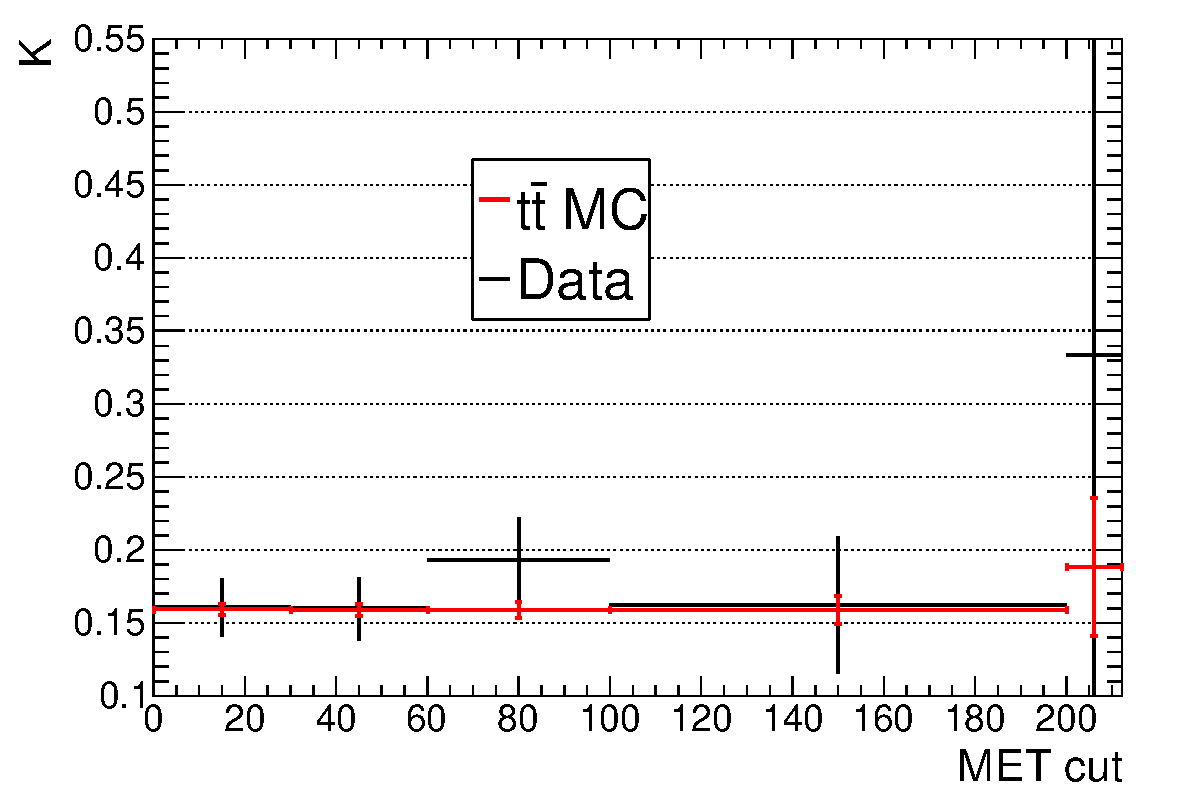
\includegraphics[width=0.48\linewidth]{plots/kvmet_data_ttbm.pdf}
%	\includegraphics[width=0.48\linewidth]{plots/kvmet_ratio.pdf}
%	\caption{
%	  \label{fig:kvmet}\protect 
%	  The left plot shows
%	  K as a function of \MET\ in MC (red) and data (black). 
%	  The bin low edge corresponds to the \MET\ cut, and the 
%	  bins are inclusive.
%	  The MC used is a sum of all SM MC used in the yield table of
%	  section \ref{sec:yields}.
%	  The right plot is the ratio of K in data to MC.
%	  The ratio is fit to a line whose slope is consistent with zero
%	  (the fit parameters are 
%	  0.9 $\pm$  0.4 for the intercept and
%      0.001 $\pm$ 0.005 for the slope).
%	}
%  \end{center}
%\end{figure}
%
%
%
%\begin{table}[htb]
%\begin{center}
%\caption{\label{fig:kvmettable} The values of K used in the OF background prediction. 
%The uncertainties shown are the total relative systematic used for the OF prediction,
%which is the systematic uncertainty from K added in quadrature with
%a 7\% uncertainty from the electron to muon efficieny ratio as assessed in the
%inclusive analysis.
%}
%\begin{tabular}{lcc}
%\hline
%\MET\ Cut    &    K        &  Relative Systematic \\
%\hline
%%the met zero row is used only for normalization of the money plot.
%%0    &  0.1   &        \\  
%30   &  0.12  &  20\%  \\  
%60   &  0.13  &  20\%  \\  
%80   &  0.12  &  20\%  \\  
%100  &  0.12  &  20\%  \\  
%150  &  0.09  &  25\%  \\  
%200  &  0.06  &  60\%  \\  
%\hline
%\end{tabular}
%\end{center}
%\end{table}

\subsection{Uncertainty from the isolated track veto}
This is the uncertainty associated with how well the isolated track
veto performance is modeled by the Monte Carlo.  This uncertainty
only applies to the fraction of dilepton BG events that have 
a second e/$\mu$ or a one prong $\tau \to h$, with 
$P_T > 10$ GeV in $|\eta| < 2.4$.  This fraction is 1/3 (THIS WAS THE
7 TEV NUMBER, CHECK).  The uncertainty for these events
is XX\% and is obtained from Tag and Probe studies of Section~\ref{sec:trkveto}

\subsubsection{Isolated Track Veto: Tag and Probe Studies}
\label{sec:trkveto}

[EVERYTHING IS 7TEV HERE, UPDATE WITH NEW RESULTS \\
ADD TABLE WITH FRACTION OF EVENTS THAT HAVE A TRUE ISOLATED TRACK]

In this section we compare the performance of the isolated track veto in data and MC using tag-and-probe studies
with samples of Z$\to$ee and Z$\to\mu\mu$. The purpose of these studies is to demonstrate that the efficiency
to satisfy the isolated track veto requirements is well-reproduced in the MC, since if this were not the case 
we would need to apply a data-to-MC scale factor in order to correctly predict the \ttll\ background. This study
addresses possible data vs. MC discrepancies for the {\bf efficiency} to identify (and reject) events with a 
second {\bf genuine} lepton (e, $\mu$, or $\tau\to$1-prong). It does not address possible data vs. MC discrepancies
in the fake rate for rejecting events without a second genuine lepton; this is handled separately in the top normalization
procedure by scaling the \ttlj\ contribution to match the data in the \mt\ peak after applying the isolated track veto. 
Furthermore, we test the data and MC
isolated track veto efficiencies for electrons and muons since we are using a Z tag-and-probe technique, but we do not
directly test the performance for hadronic tracks from $\tau$ decays. The performance for hadronic $\tau$ decay products
may differ from that of electrons and muons for two reasons. First, the $\tau$ may decay to a hadronic track plus one
or two $\pi^0$'s, which may decay to $\gamma\gamma$ followed by a photon conversion. As shown in Figure~\ref{fig:absiso},
the isolation distribution for charged tracks from $\tau$ decays that are not produced in association with $\pi^0$s are 
consistent with that from $\E$s and $\M$s. Since events from single prong $\tau$ decays produced in association with 
$\pi^0$s comprise a small fraction of the total sample, and since the kinematics of $\tau$, $\pi^0$ and $\gamma\to e^+e^-$
decays are well-understood, we currently demonstrate that the isolation is well-reproduced for electrons and muons only.
Second, hadronic tracks may undergo nuclear interactions and hence their tracks may not be reconstructed.
As discussed above, independent studies show that the MC reproduces the hadronic tracking efficiency within 4\%,
leading to a total background uncertainty of less than 0.5\% (after taking into account the fraction of the total background
due to hadronic $\tau$ decays with \pt\ $>$ 10 GeV tracks), and we hence regard this effect as neglgigible.

The tag-and-probe studies are performed in the full 2011 data sample, and compared with the DYJets madgraph sample.
All events must contain a tag-probe pair (details below) with opposite-sign and satisfying the Z mass requirement 76--106 GeV.
We compare the distributions of absolute track isolation for probe electrons/muons in data vs. MC. The contributions to
this isolation sum are from ambient energy in the event from underlying event, pile-up and jet activitiy, and hence do
not depend on the \pt\ of the probe lepton. We therefore restrict the probe \pt\ to be $>$ 30 GeV in order to suppress
fake backgrounds with steeply-falling \pt\ spectra. To suppress non-Z backgrounds (in particular \ttbar) we require 
\met\ $<$ 30 GeV and 0 b-tagged events. 
The specific criteria for tags and probes for electrons and muons are:

%We study the isolated track veto efficiency in bins of \njets.
%We are interested in events with at least 4 jets to emulate the hadronic activity in our signal sample. However since
%there are limited statistics for Z + $\geq$4 jet events, we study the isolated track performance in events with


\begin{itemize}
  \item{Electrons}

    \begin{itemize}
    \item{Tag criteria}

      \begin{itemize}
      \item Electron passes full analysis ID/iso selection 
      \item \pt\ $>$ 30 GeV, $|\eta|<2.5$
 
      \item Matched to 1 of the 2 electron tag-and-probe triggers
        \begin{itemize}
        \item \verb=HLT_Ele17_CaloIdVT_CaloIsoVT_TrkIdT_TrkIsoVT_SC8_Mass30_v*=
        \item \verb=HLT_Ele17_CaloIdVT_CaloIsoVT_TrkIdT_TrkIsoVT_Ele8_Mass30_v*=
        \end{itemize}
      \end{itemize}

    \item{Probe criteria}
      \begin{itemize}
      \item Electron passes full analysis ID selection
      \item \pt\ $>$ 30 GeV
      \end{itemize}
      \end{itemize}
  \item{Muons}
    \begin{itemize}
    \item{Tag criteria}
      \begin{itemize}
      \item Muon passes full analysis ID/iso selection
      \item \pt\ $>$ 30 GeV, $|\eta|<2.1$
      \item Matched to 1 of the 2 electron tag-and-probe triggers
        \begin{itemize}
        \item \verb=HLT_IsoMu30_v*=
        \item \verb=HLT_IsoMu30_eta2p1_v*=
        \end{itemize}
      \end{itemize}
    \item{Probe criteria}
      \begin{itemize}
      \item Muon passes full analysis ID selection
      \item \pt\ $>$ 30 GeV
      \end{itemize}
    \end{itemize}
\end{itemize}

The absolute track isolation distributions for passing probes are displayed in Fig.~\ref{fig:tnp}. In general we observe
good agreement between data and MC. To be more quantitative, we compare the data vs. MC efficiencies to satisfy
absolute track isolation requirements varying from $>$ 1 GeV to $>$ 5 GeV, as summarized in Table~\ref{tab:isotrk}.
In the $\geq$0 and $\geq$1 jet bins where the efficiencies can be tested with statistical precision, the data and MC
efficiencies agree within 7\%, and we apply this as a systematic uncertainty on the isolated track veto efficiency.
For the higher jet multiplicity bins the statistical precision decreases, but we do not observe any evidence for
a data vs. MC discrepancy in the isolated track veto efficiency.


%This is because our analysis requirement is relative track isolation $<$ 0.1, and m
%This requirement is chosen because most of the tracks rejected by the isolated
%track veto have a \pt\ near the 10 GeV threshold, and our analysis requirement is relative track isolation $<$ 1 GeV.

\begin{figure}[hbt]
  \begin{center}
	%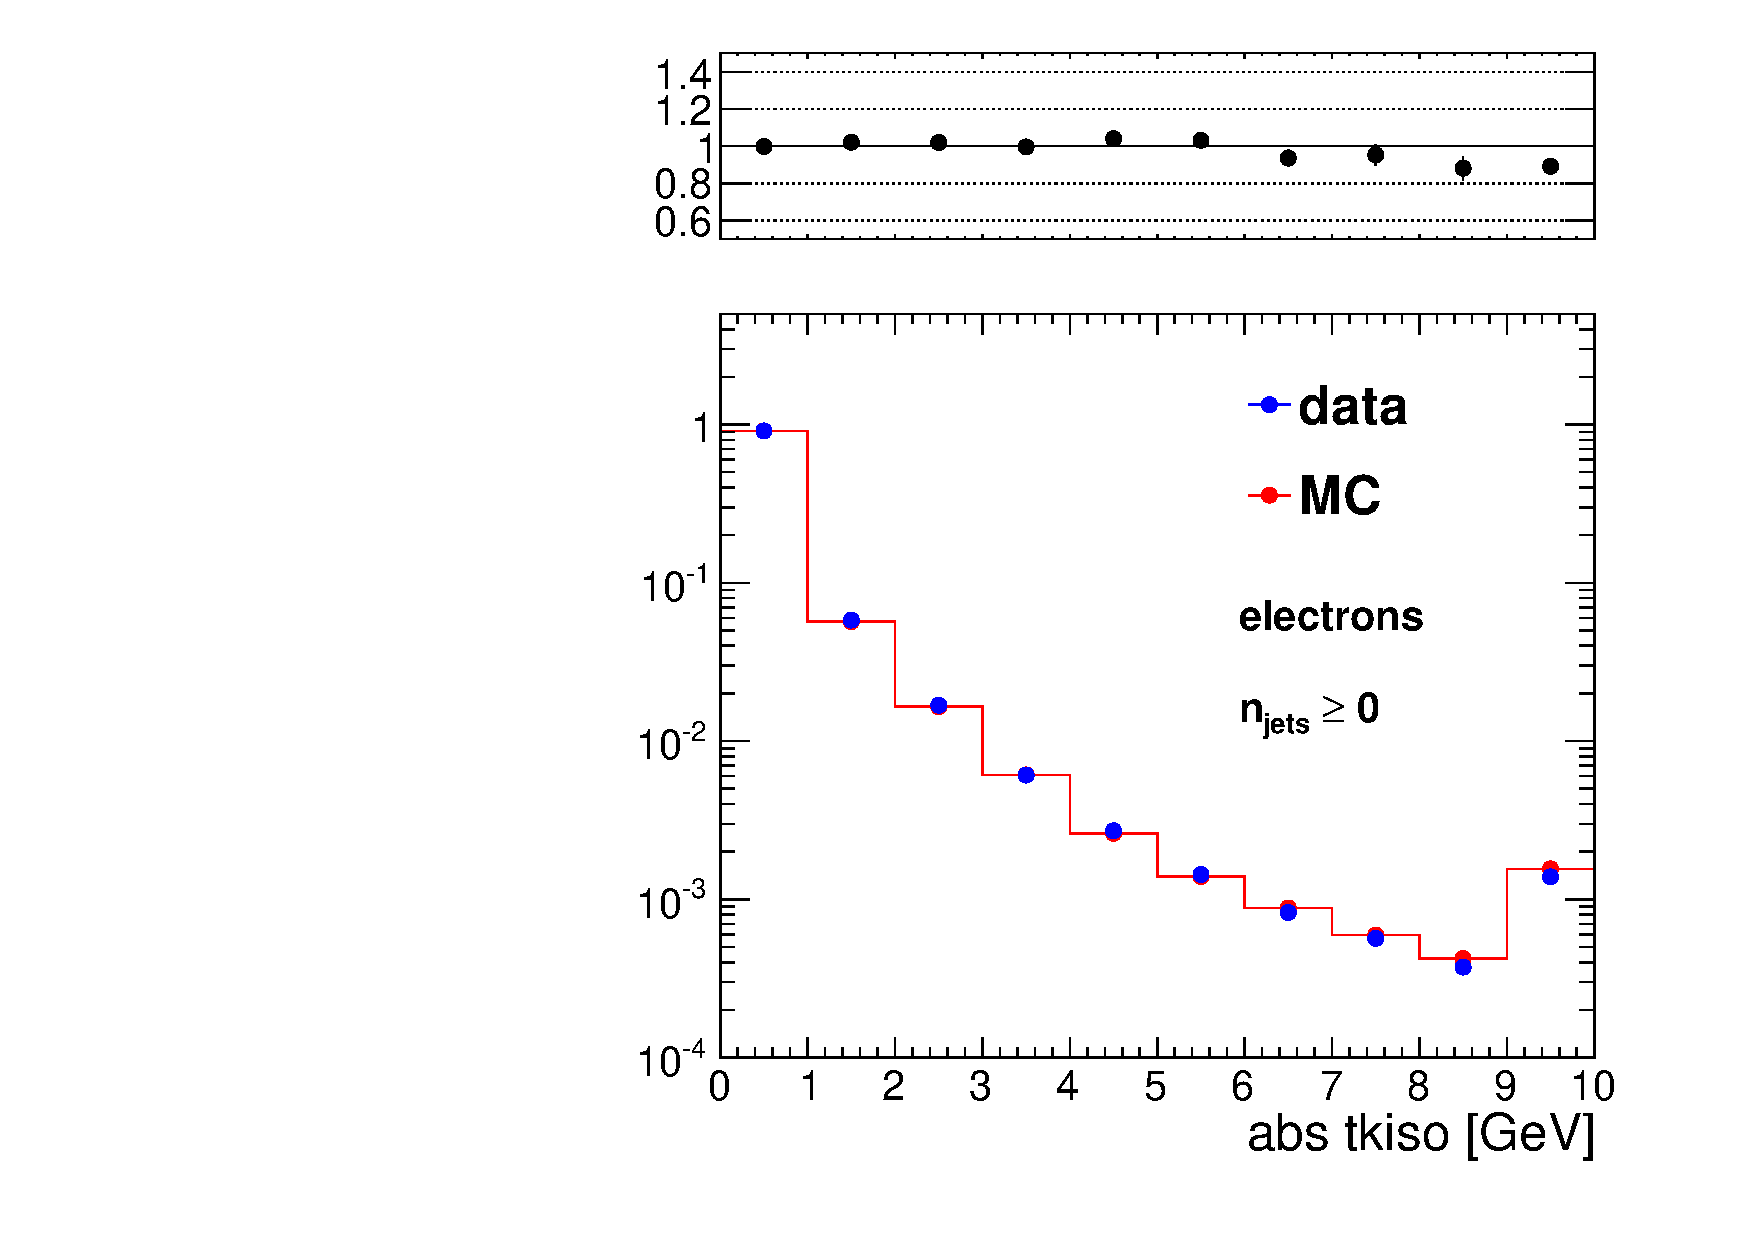
\includegraphics[width=0.3\linewidth]{plots/el_tkiso_0j.pdf}%
	%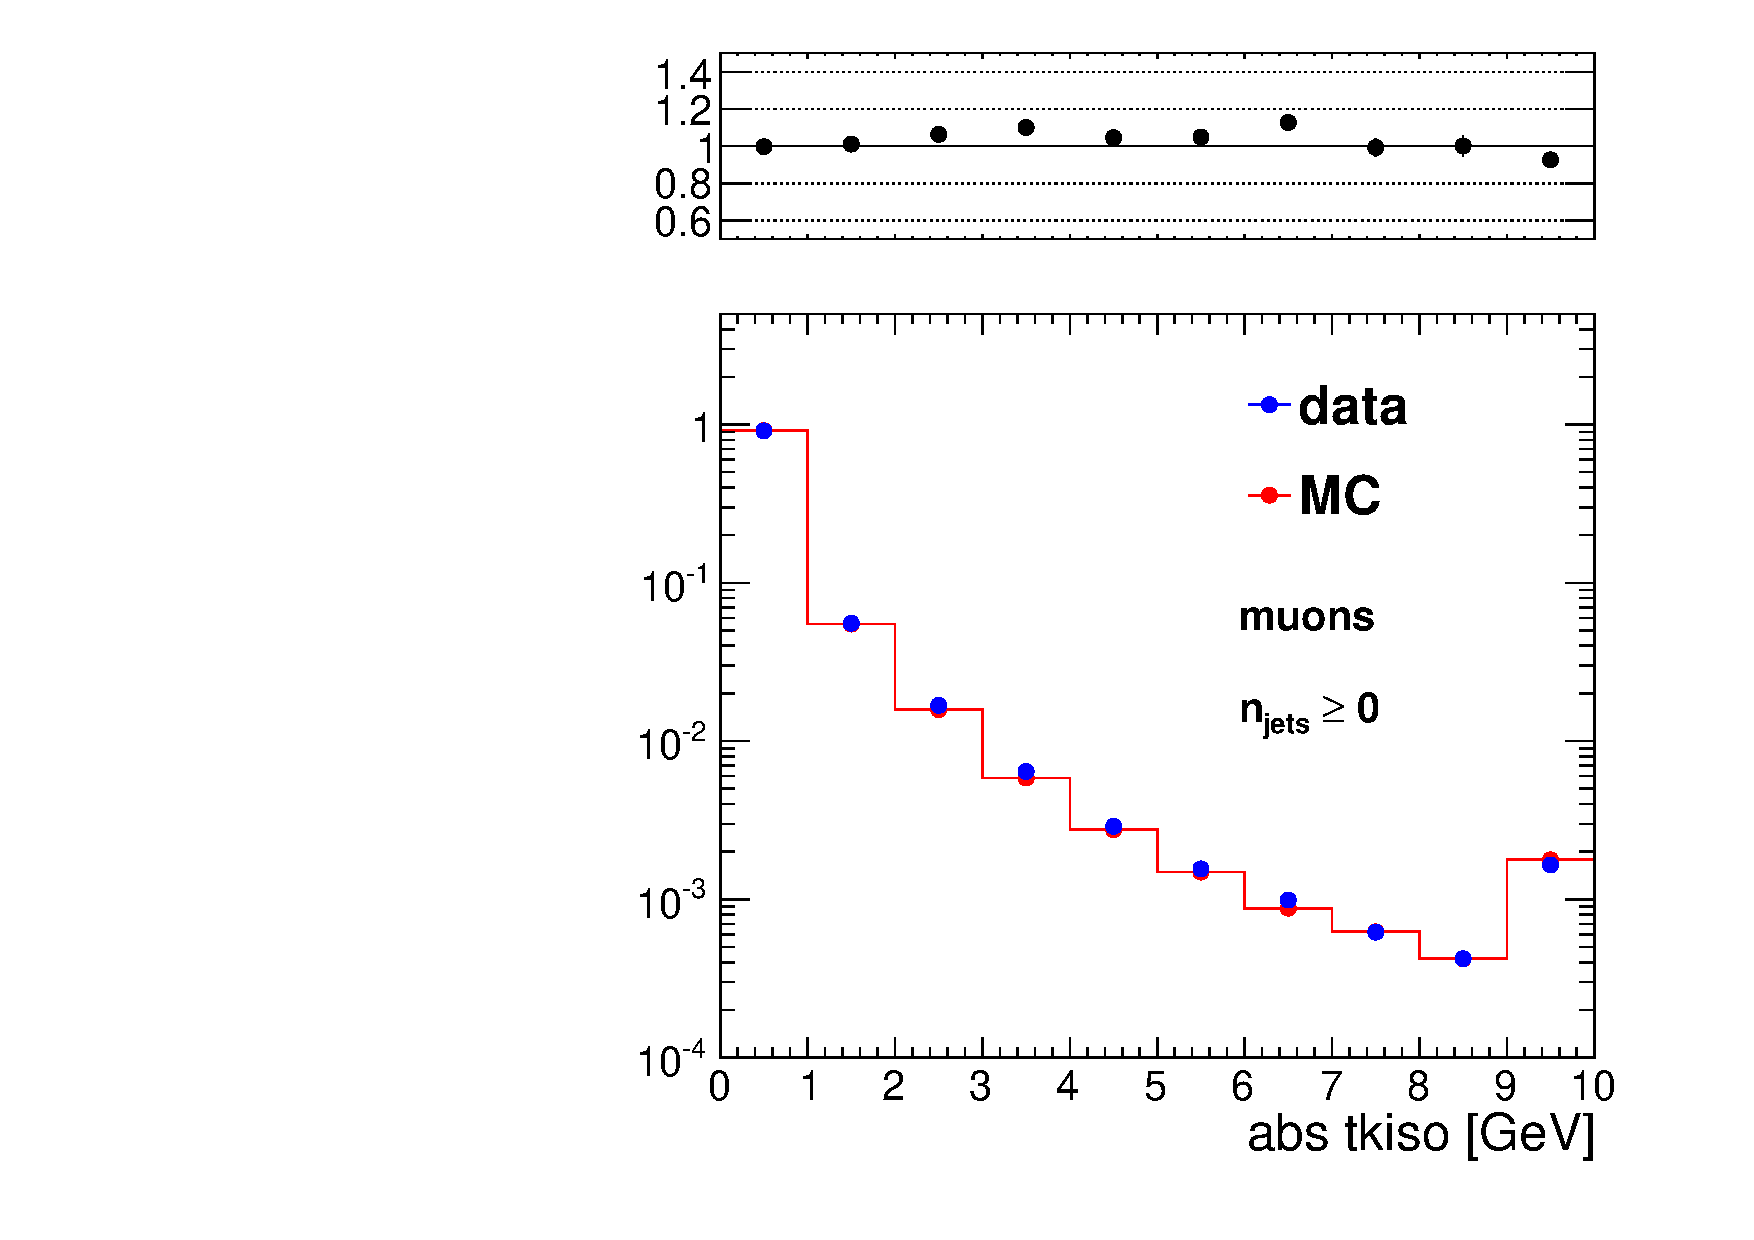
\includegraphics[width=0.3\linewidth]{plots/mu_tkiso_0j.pdf}
	%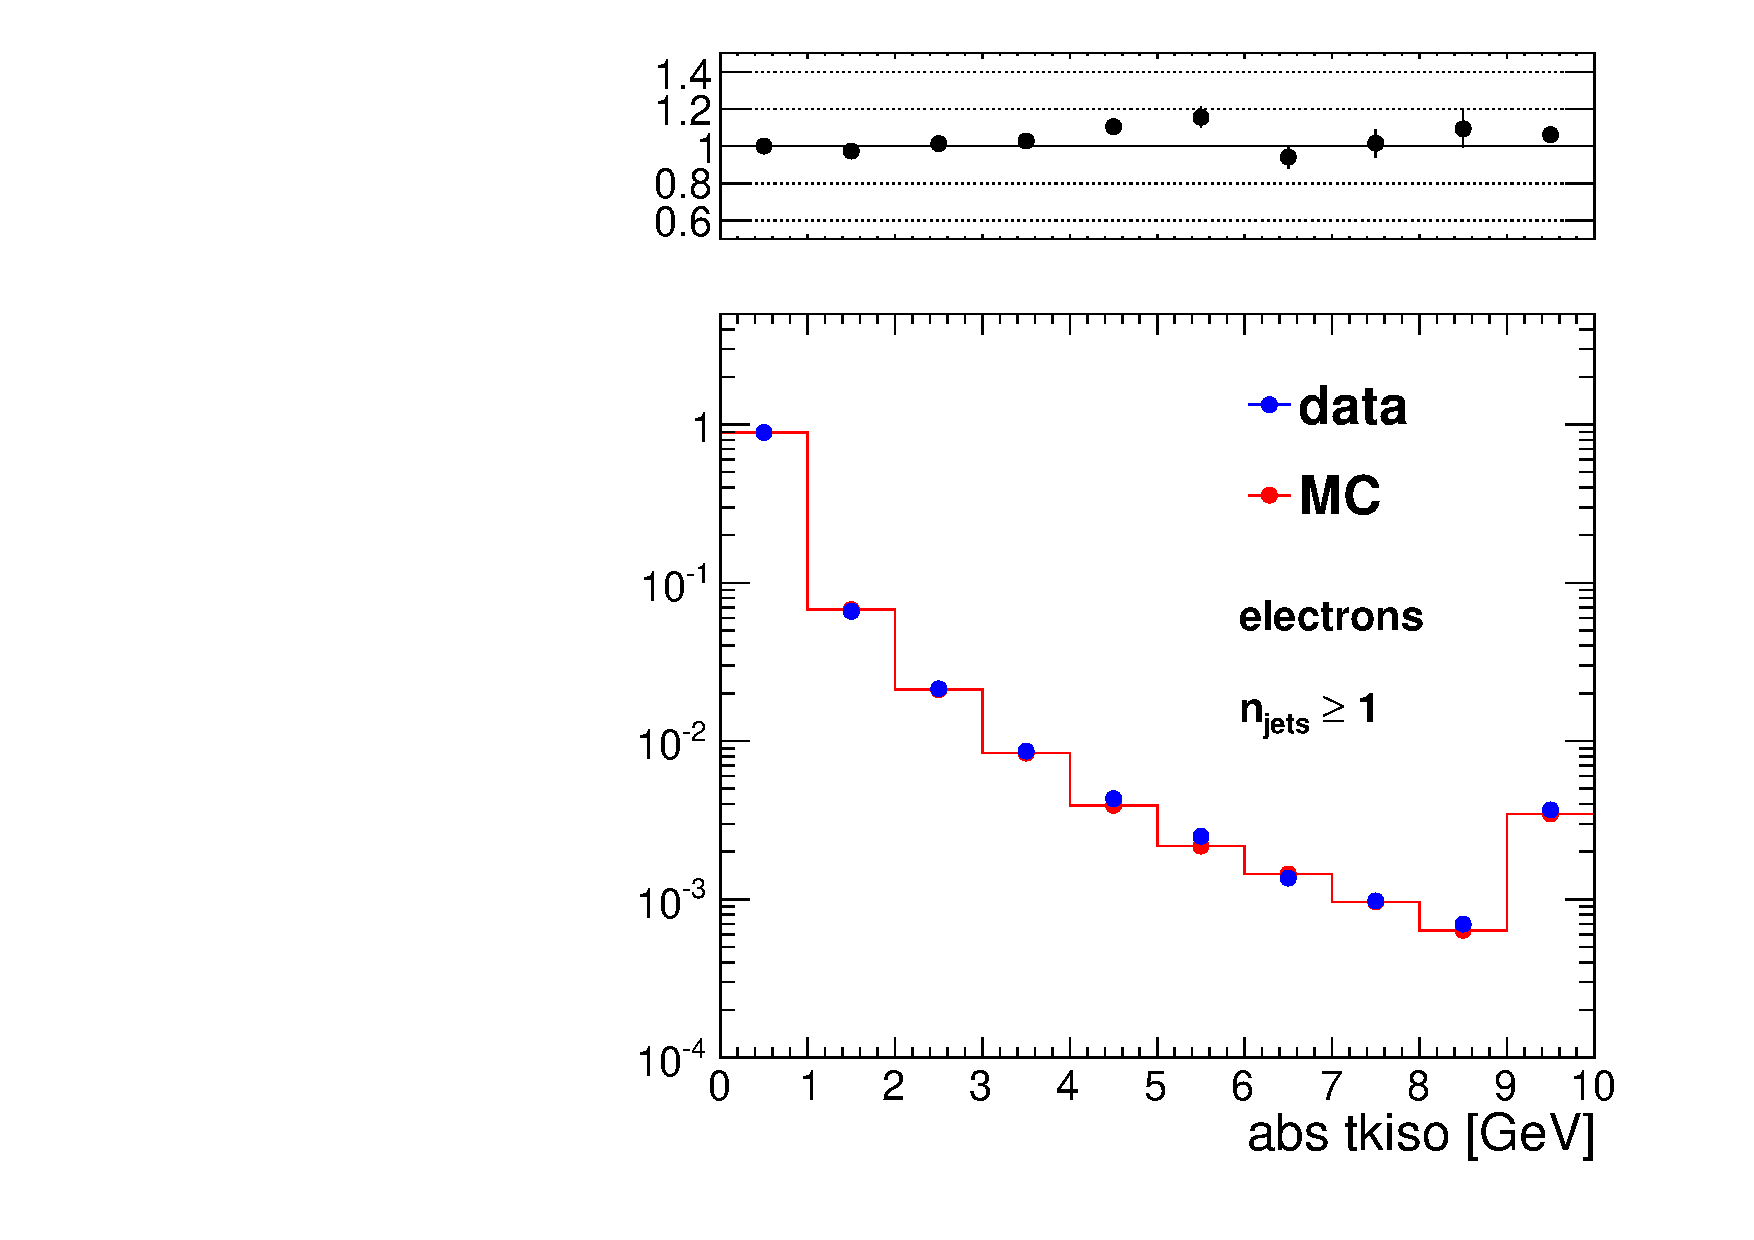
\includegraphics[width=0.3\linewidth]{plots/el_tkiso_1j.pdf}%
	%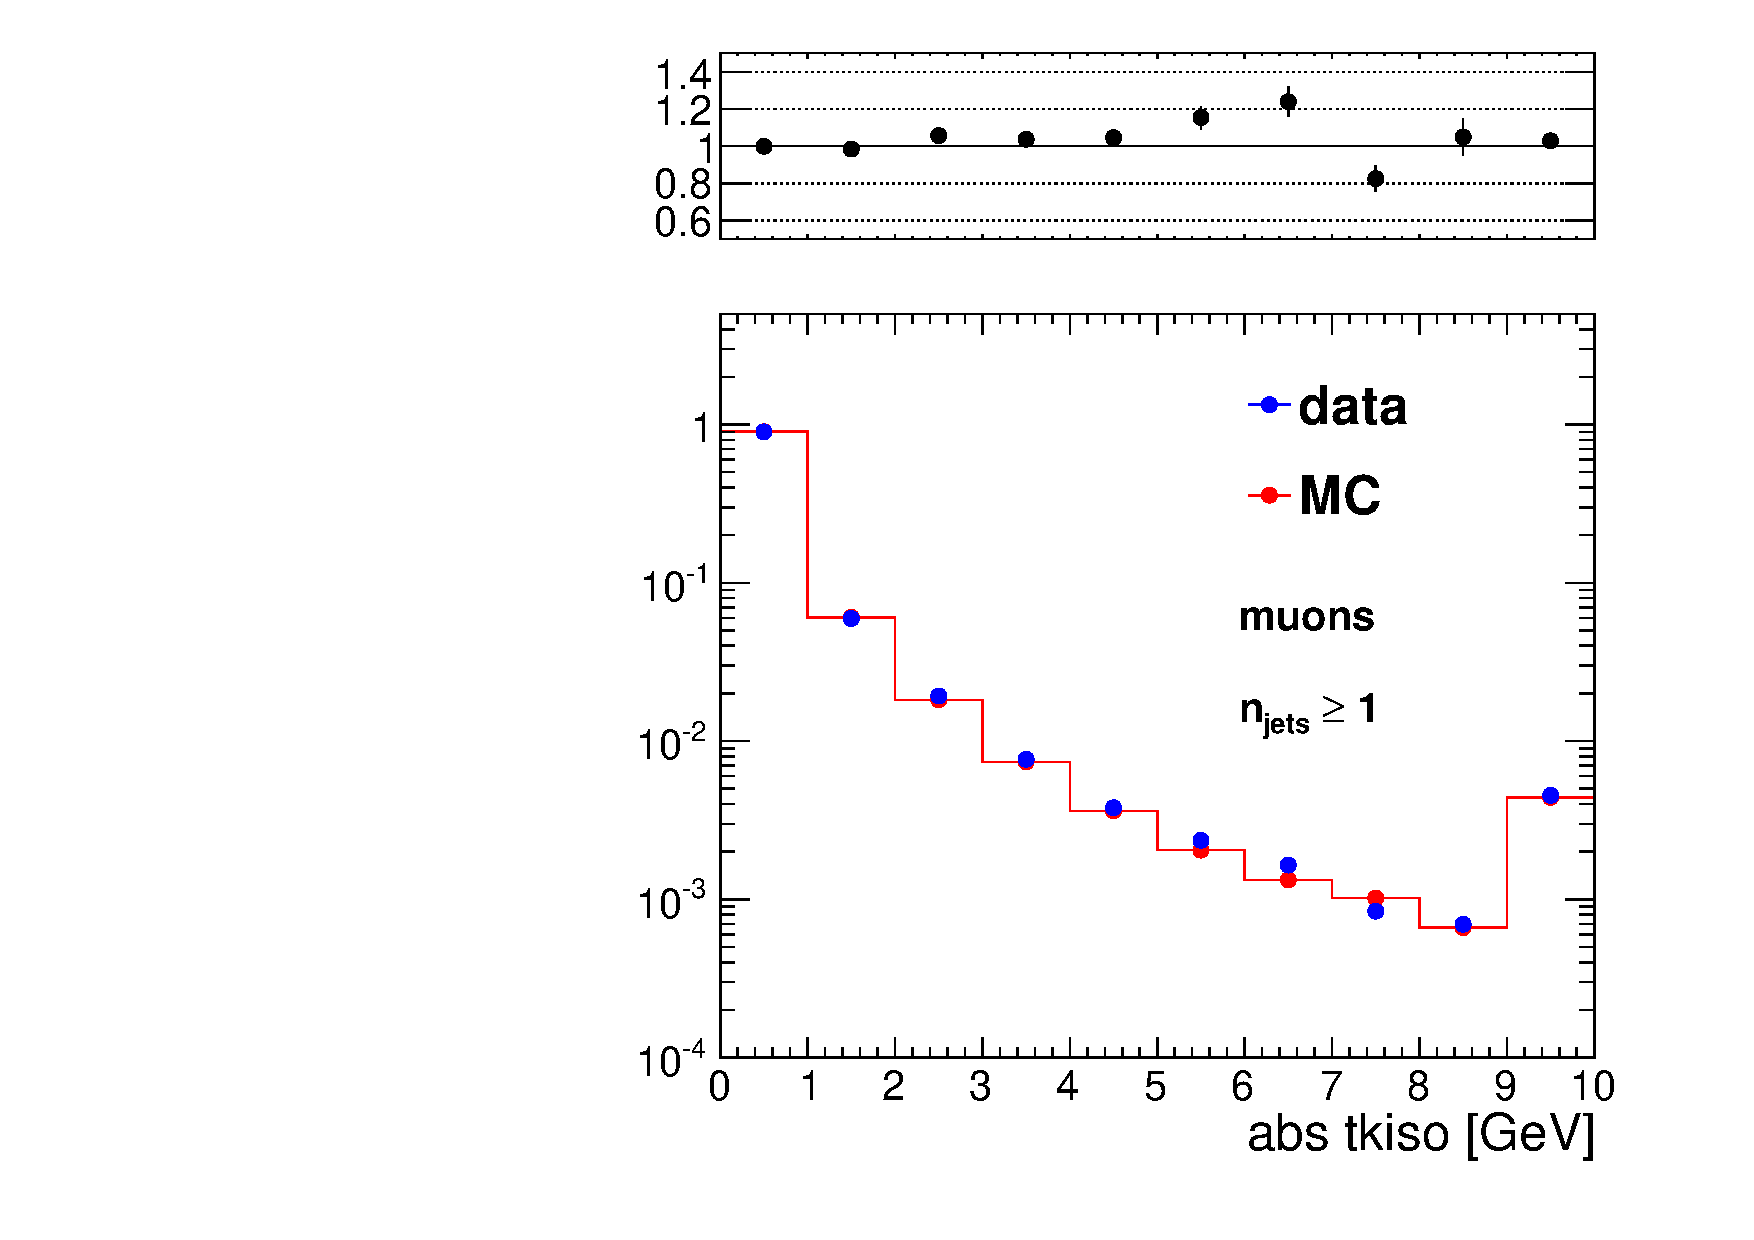
\includegraphics[width=0.3\linewidth]{plots/mu_tkiso_1j.pdf}
	%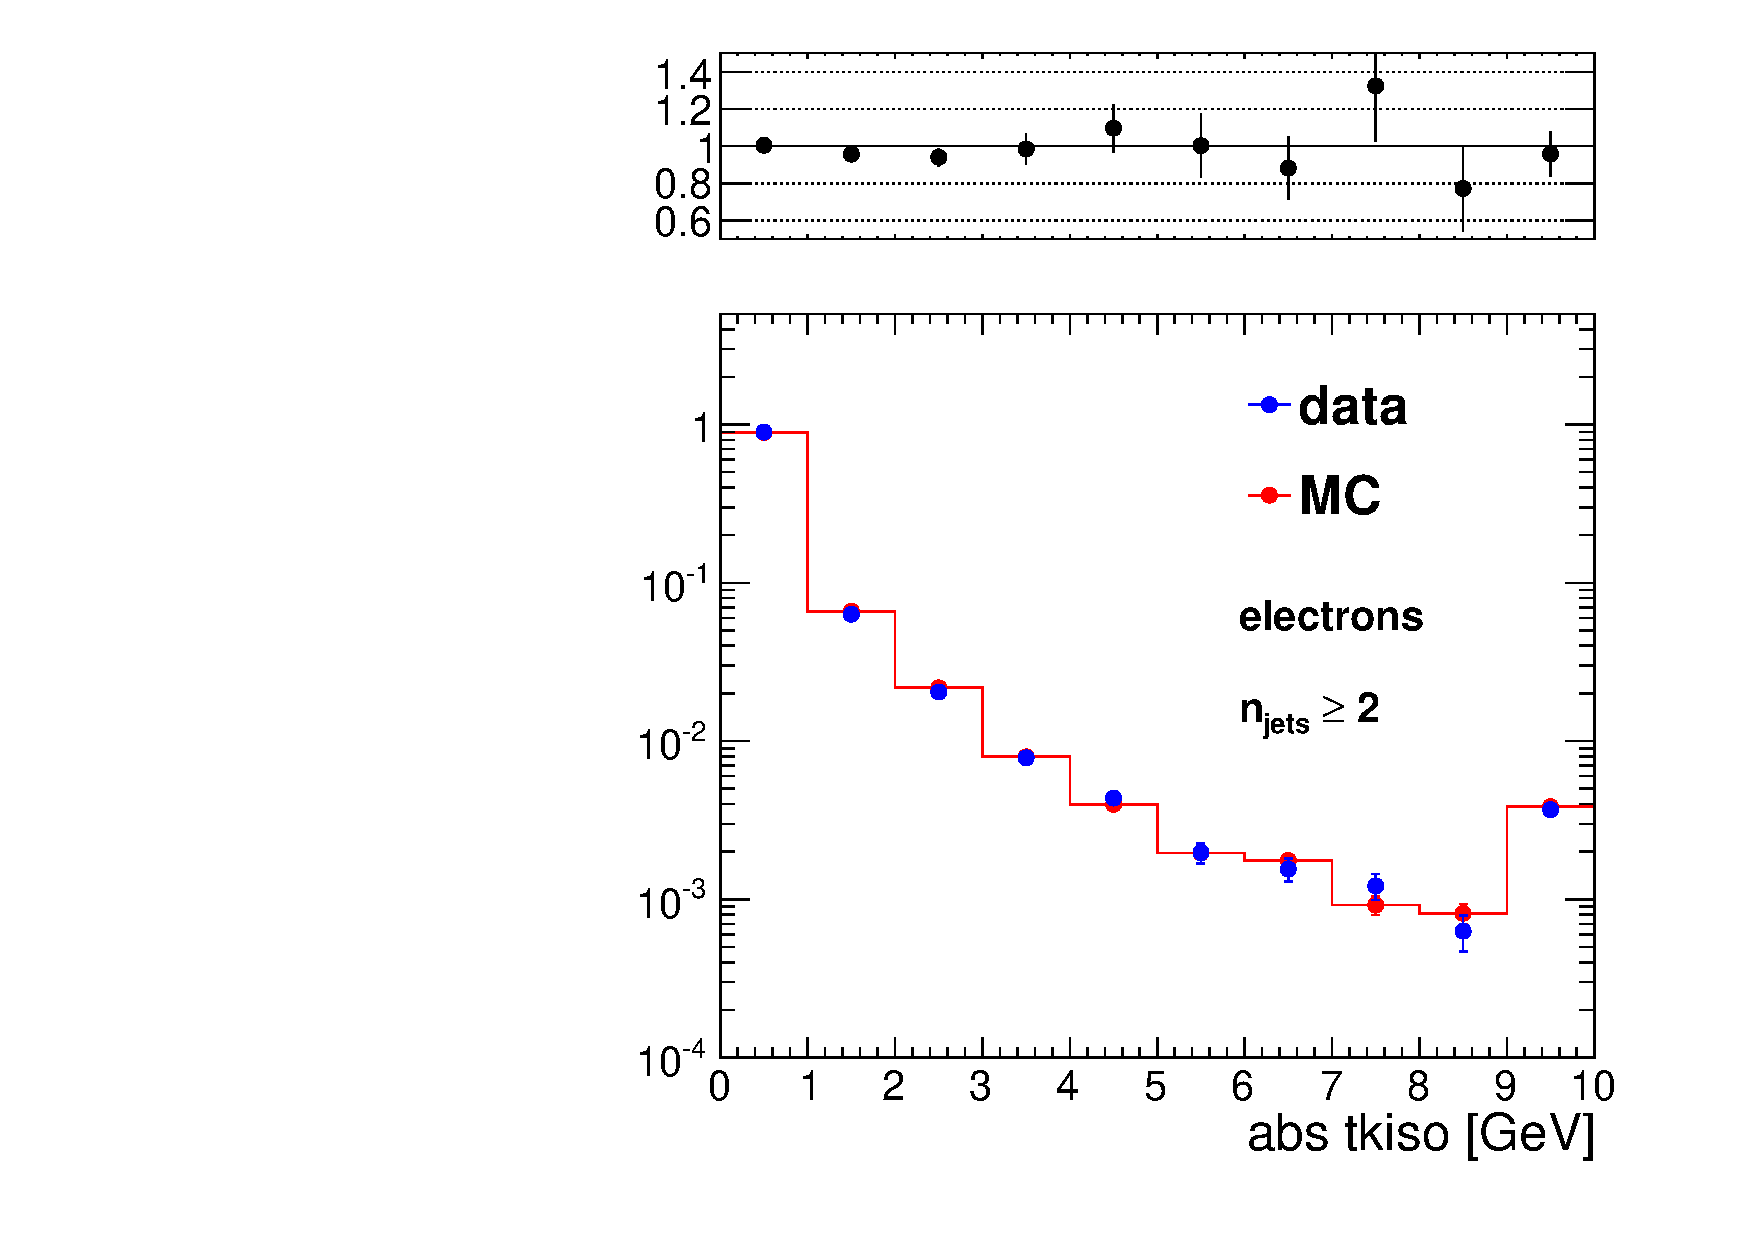
\includegraphics[width=0.3\linewidth]{plots/el_tkiso_2j.pdf}%
	%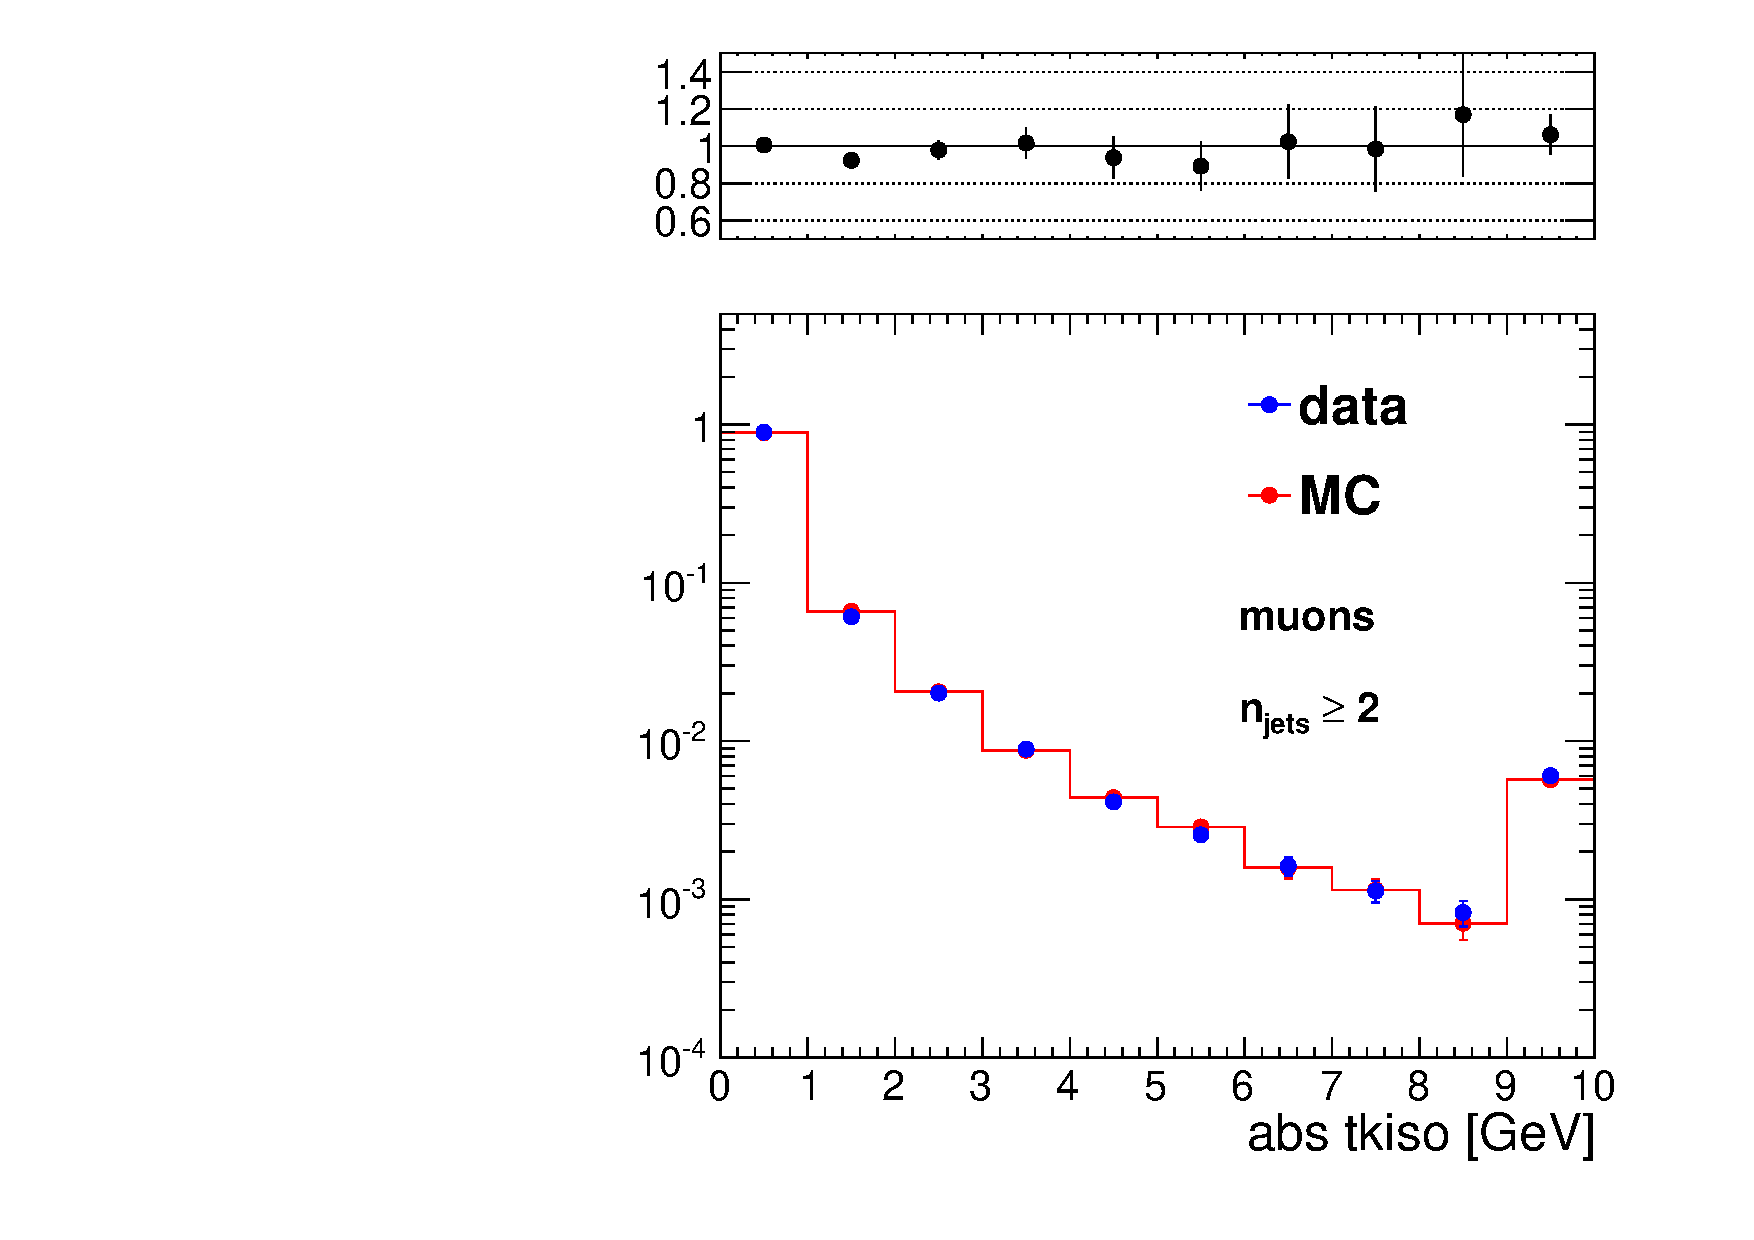
\includegraphics[width=0.3\linewidth]{plots/mu_tkiso_2j.pdf}
	%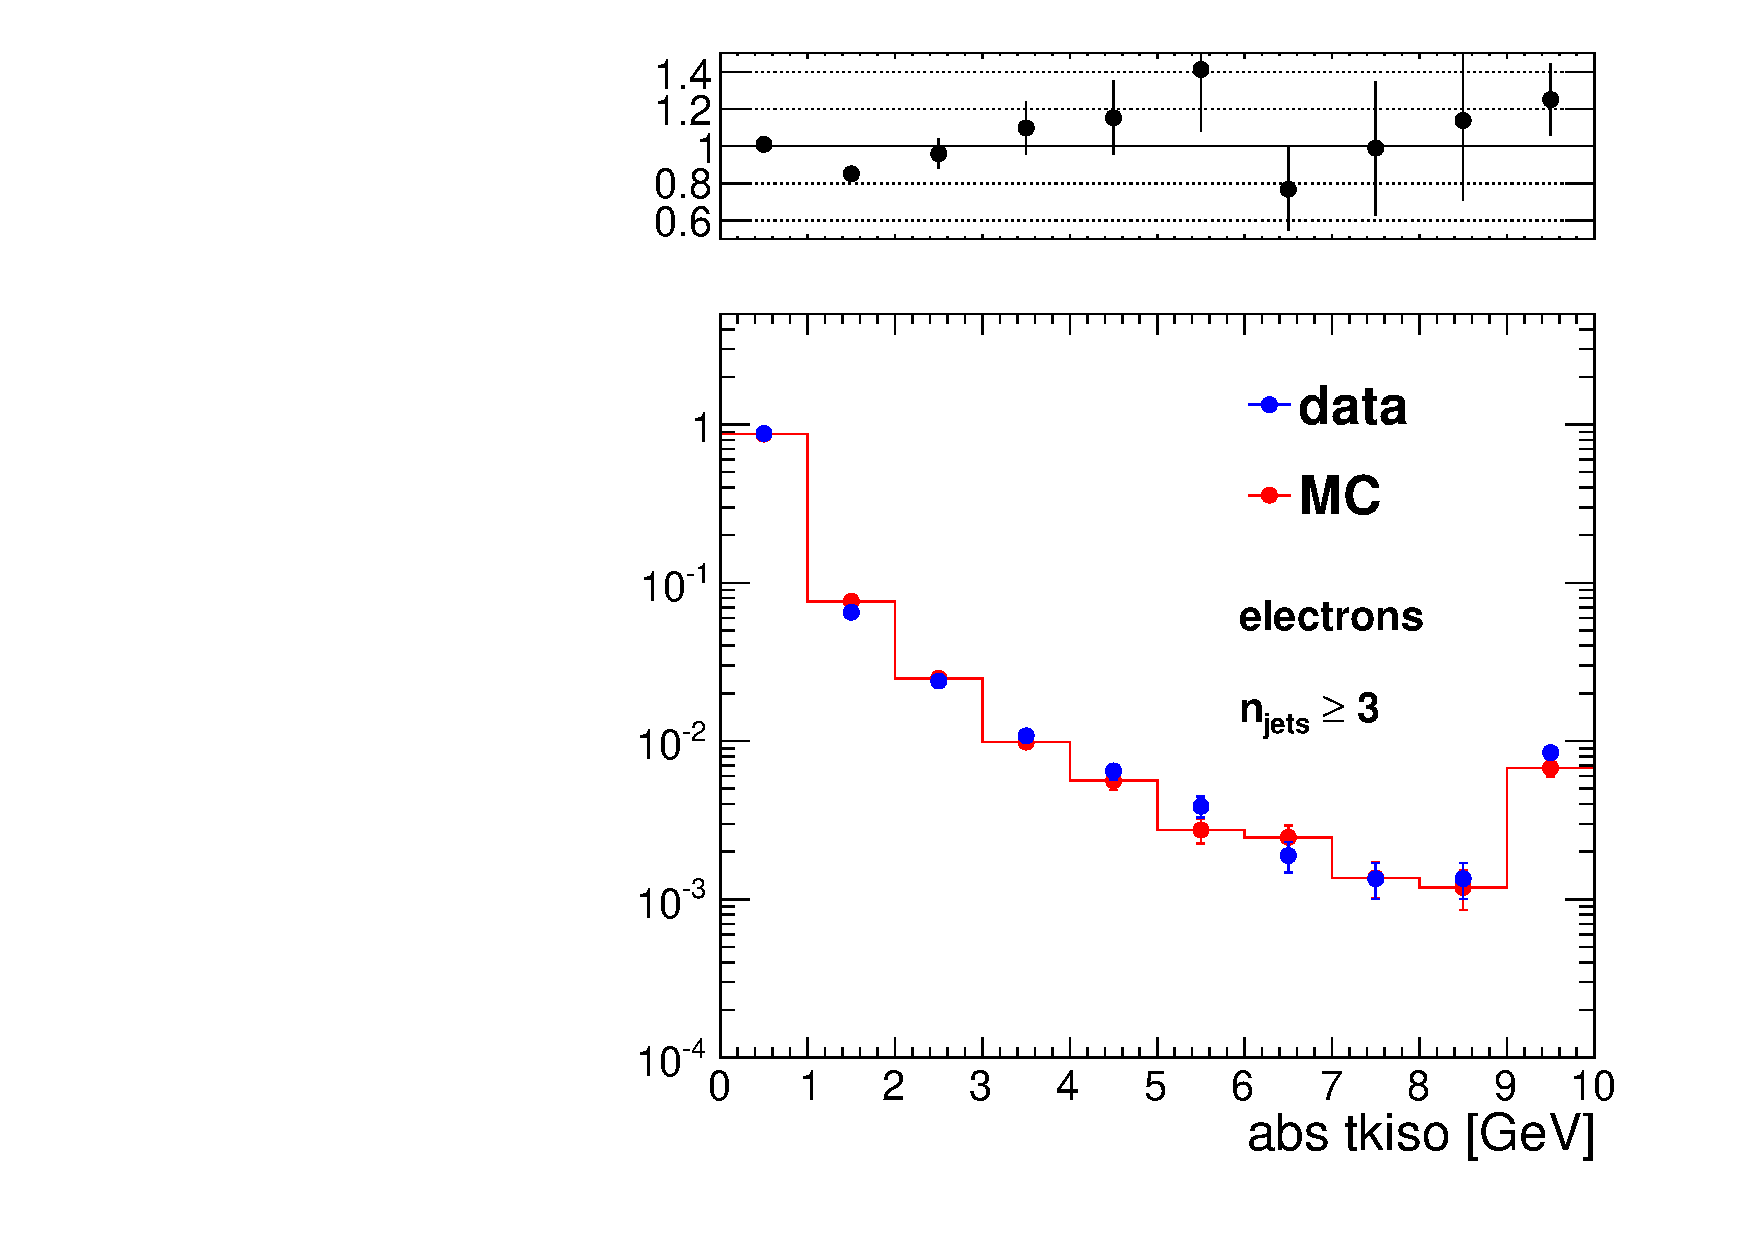
\includegraphics[width=0.3\linewidth]{plots/el_tkiso_3j.pdf}%
	%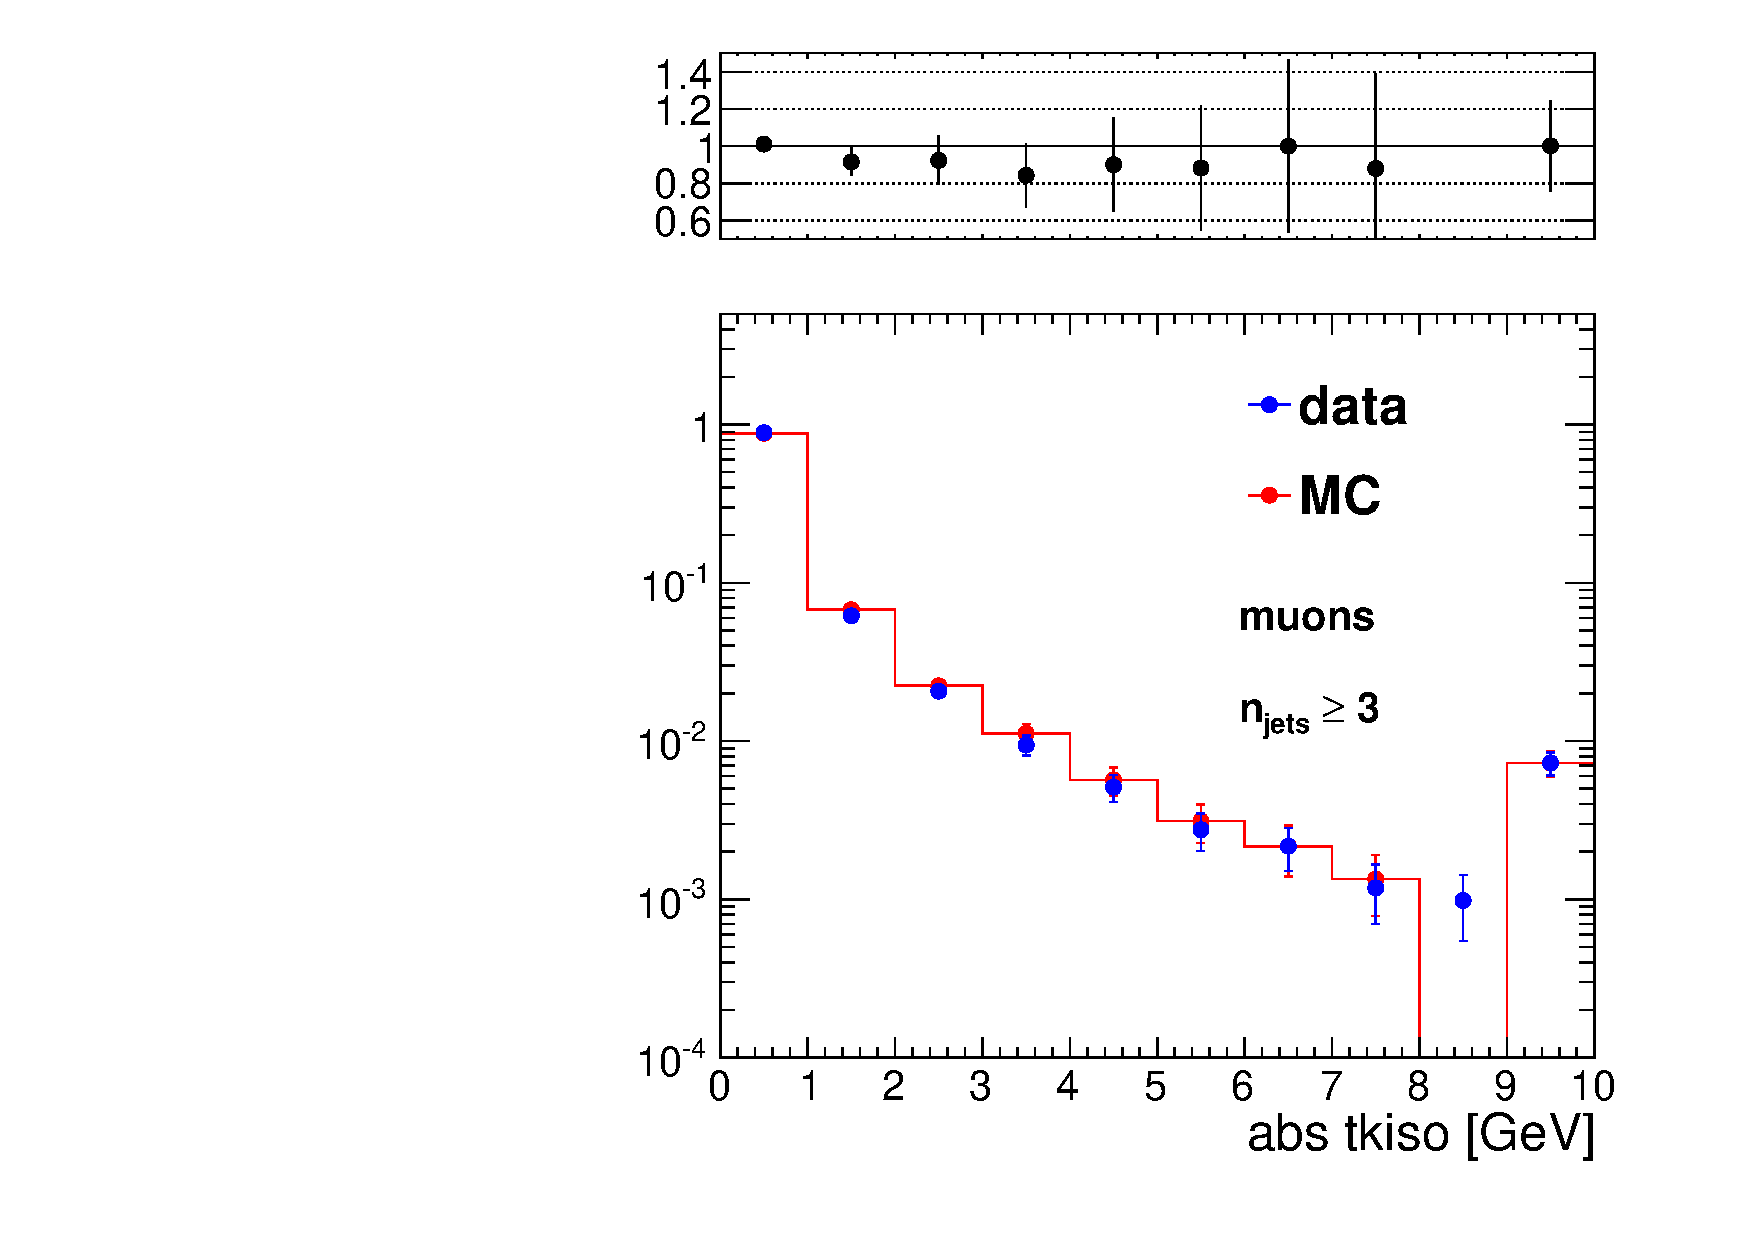
\includegraphics[width=0.3\linewidth]{plots/mu_tkiso_3j.pdf}
	%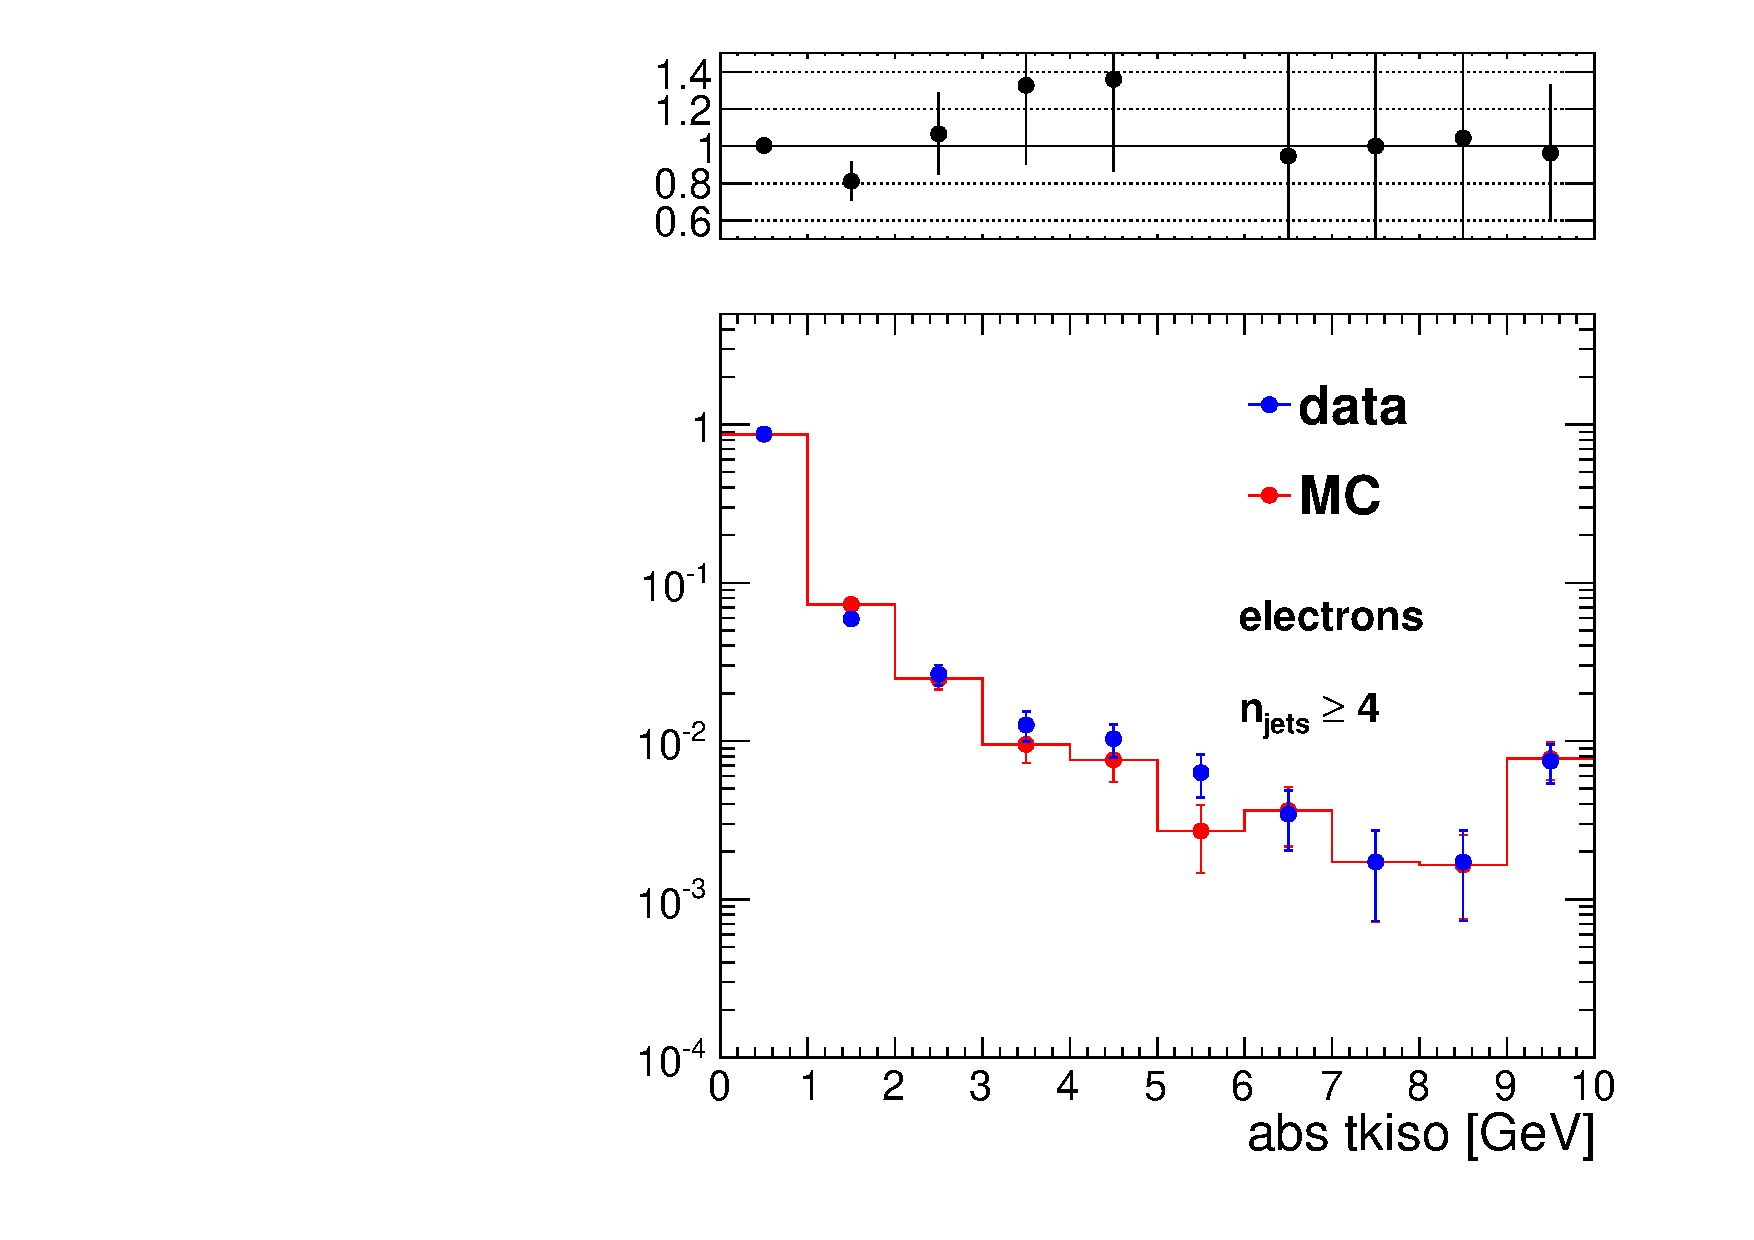
\includegraphics[width=0.3\linewidth]{plots/el_tkiso_4j.pdf}%
	%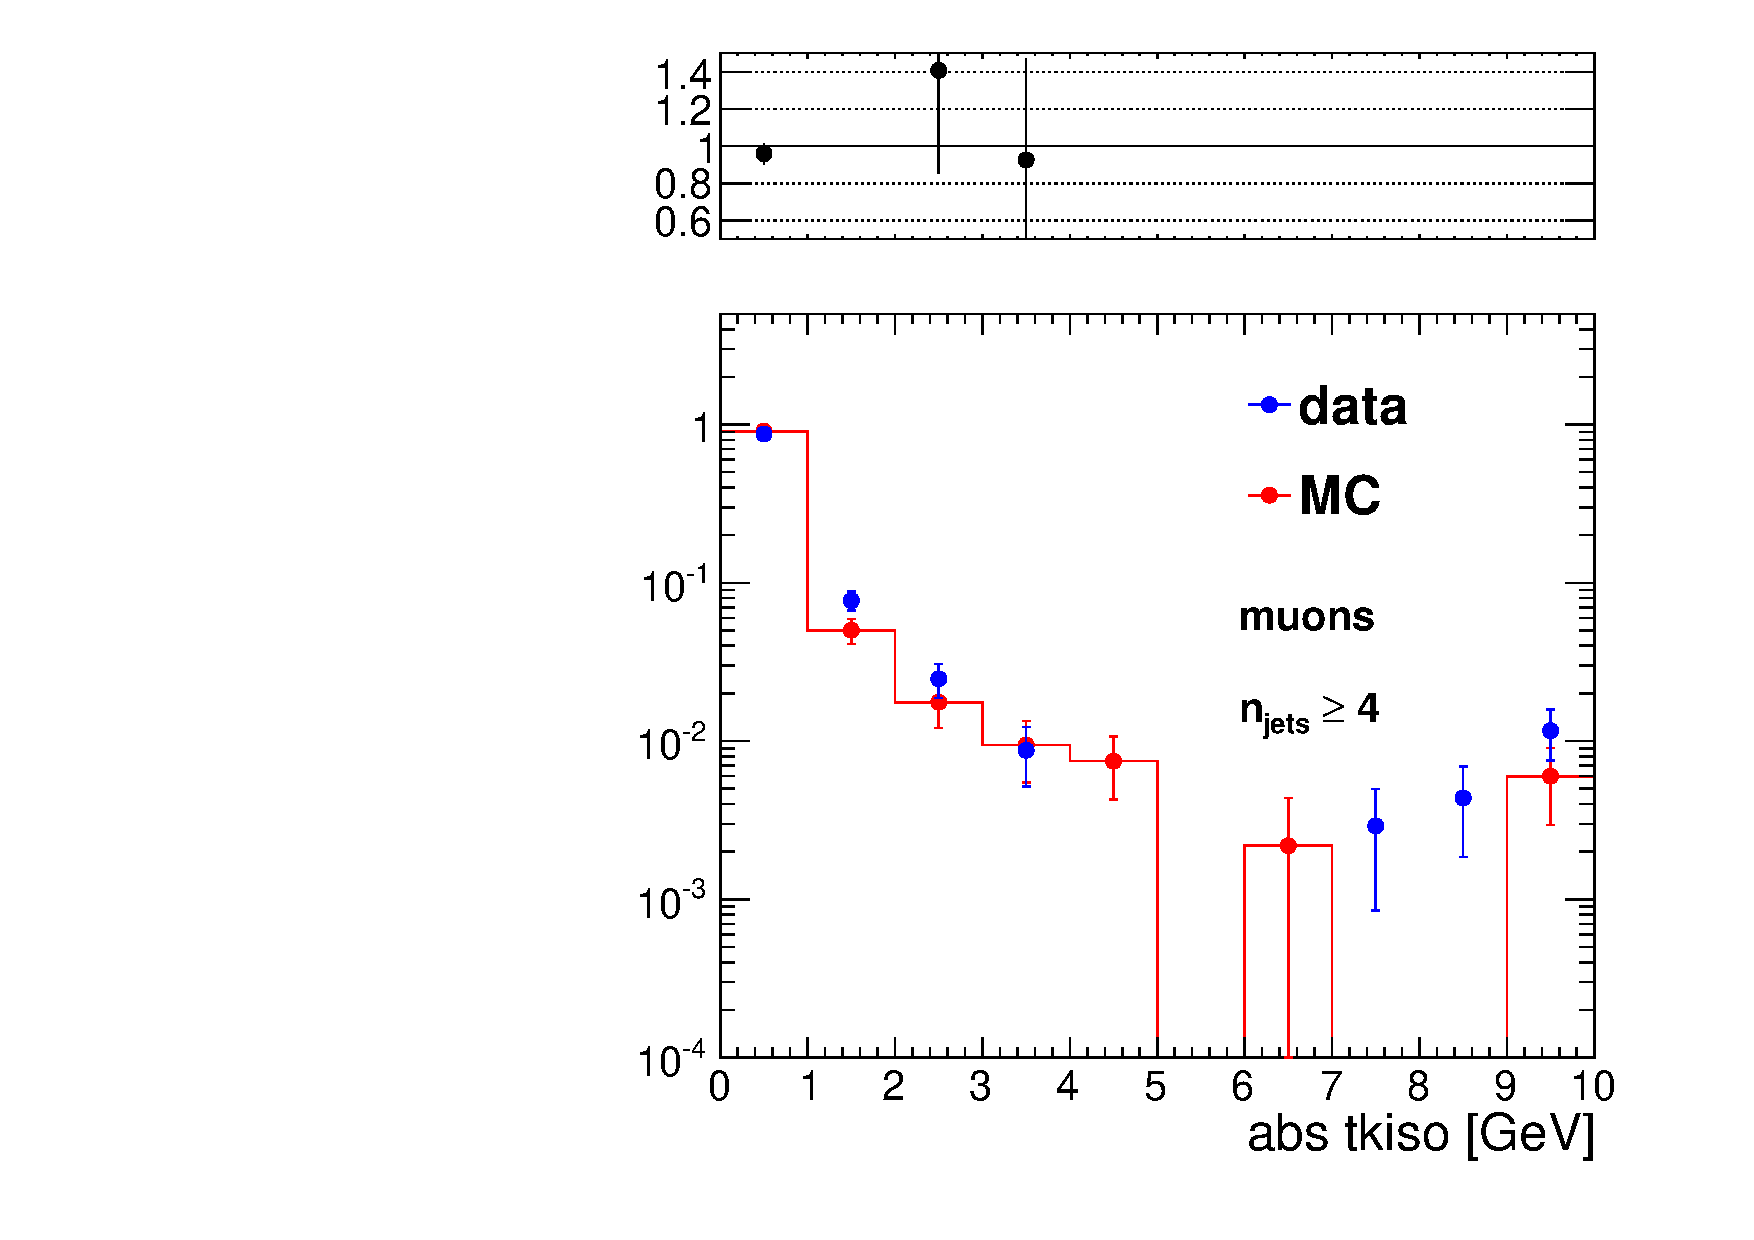
\includegraphics[width=0.3\linewidth]{plots/mu_tkiso_4j.pdf}
	\caption{
	  \label{fig:tnp} Comparison of the absolute track isolation in data vs. MC for electrons (left) and muons (right)
for events with the \njets\ requirement varied from \njets\ $\geq$ 0 to \njets\ $\geq$ 4. 
}  
      \end{center}
\end{figure}

\clearpage

\begin{table}[!ht]
\begin{center}
\caption{\label{tab:isotrk} Comparison of the data vs. MC efficiencies to satisfy the indicated requirements
on the absolute track isolation, and the ratio of these two efficiencies. Results are indicated separately for electrons and muons and for various
jet multiplicity requirements.}
\begin{tabular}{l|l|c|c|c|c|c}
\hline
\hline
 e + $\geq$0 jets            &           $>$ 1 GeV   &           $>$ 2 GeV   &           $>$ 3 GeV   &           $>$ 4 GeV   &           $>$ 5 GeV  \\
\hline
      data   &  0.088 $\pm$ 0.0003   &  0.030 $\pm$ 0.0002   &  0.013 $\pm$ 0.0001   &  0.007 $\pm$ 0.0001   &  0.005 $\pm$ 0.0001  \\
        mc   &  0.087 $\pm$ 0.0001   &  0.030 $\pm$ 0.0001   &  0.014 $\pm$ 0.0001   &  0.008 $\pm$ 0.0000   &  0.005 $\pm$ 0.0000  \\
   data/mc   &     1.01 $\pm$ 0.00   &     0.99 $\pm$ 0.01   &     0.97 $\pm$ 0.01   &     0.95 $\pm$ 0.01   &     0.93 $\pm$ 0.01  \\
\hline
\hline
 $\mu$ + $\geq$0 jets            &           $>$ 1 GeV   &           $>$ 2 GeV   &           $>$ 3 GeV   &           $>$ 4 GeV   &           $>$ 5 GeV  \\
\hline
      data   &  0.087 $\pm$ 0.0002   &  0.031 $\pm$ 0.0001   &  0.015 $\pm$ 0.0001   &  0.008 $\pm$ 0.0001   &  0.005 $\pm$ 0.0001  \\
        mc   &  0.085 $\pm$ 0.0001   &  0.030 $\pm$ 0.0001   &  0.014 $\pm$ 0.0000   &  0.008 $\pm$ 0.0000   &  0.005 $\pm$ 0.0000  \\
   data/mc   &     1.02 $\pm$ 0.00   &     1.06 $\pm$ 0.00   &     1.06 $\pm$ 0.01   &     1.03 $\pm$ 0.01   &     1.02 $\pm$ 0.01  \\
\hline
\hline 
 e + $\geq$1 jets            &           $>$ 1 GeV   &           $>$ 2 GeV   &           $>$ 3 GeV   &           $>$ 4 GeV   &           $>$ 5 GeV  \\
\hline
      data   &  0.099 $\pm$ 0.0008   &  0.038 $\pm$ 0.0005   &  0.019 $\pm$ 0.0004   &  0.011 $\pm$ 0.0003   &  0.008 $\pm$ 0.0002  \\
        mc   &  0.100 $\pm$ 0.0004   &  0.038 $\pm$ 0.0003   &  0.019 $\pm$ 0.0002   &  0.012 $\pm$ 0.0002   &  0.008 $\pm$ 0.0001  \\
   data/mc   &     0.99 $\pm$ 0.01   &     1.00 $\pm$ 0.02   &     0.99 $\pm$ 0.02   &     0.98 $\pm$ 0.03   &     0.97 $\pm$ 0.03  \\
\hline
\hline
 $\mu$ + $\geq$1 jets            &           $>$ 1 GeV   &           $>$ 2 GeV   &           $>$ 3 GeV   &           $>$ 4 GeV   &           $>$ 5 GeV  \\
\hline
      data   &  0.100 $\pm$ 0.0006   &  0.041 $\pm$ 0.0004   &  0.022 $\pm$ 0.0003   &  0.014 $\pm$ 0.0002   &  0.010 $\pm$ 0.0002  \\
        mc   &  0.099 $\pm$ 0.0004   &  0.039 $\pm$ 0.0002   &  0.020 $\pm$ 0.0002   &  0.013 $\pm$ 0.0001   &  0.009 $\pm$ 0.0001  \\
   data/mc   &     1.01 $\pm$ 0.01   &     1.05 $\pm$ 0.01   &     1.05 $\pm$ 0.02   &     1.06 $\pm$ 0.02   &     1.06 $\pm$ 0.03  \\
\hline
\hline
 e + $\geq$2 jets            &           $>$ 1 GeV   &           $>$ 2 GeV   &           $>$ 3 GeV   &           $>$ 4 GeV   &           $>$ 5 GeV  \\
\hline
      data   &  0.105 $\pm$ 0.0020   &  0.042 $\pm$ 0.0013   &  0.021 $\pm$ 0.0009   &  0.013 $\pm$ 0.0007   &  0.009 $\pm$ 0.0006  \\
        mc   &  0.109 $\pm$ 0.0011   &  0.043 $\pm$ 0.0007   &  0.021 $\pm$ 0.0005   &  0.013 $\pm$ 0.0004   &  0.009 $\pm$ 0.0003  \\
   data/mc   &     0.96 $\pm$ 0.02   &     0.97 $\pm$ 0.03   &     1.00 $\pm$ 0.05   &     1.01 $\pm$ 0.06   &     0.97 $\pm$ 0.08  \\
\hline
\hline
 $\mu$ + $\geq$2 jets            &           $>$ 1 GeV   &           $>$ 2 GeV   &           $>$ 3 GeV   &           $>$ 4 GeV   &           $>$ 5 GeV  \\
\hline
      data   &  0.106 $\pm$ 0.0016   &  0.045 $\pm$ 0.0011   &  0.025 $\pm$ 0.0008   &  0.016 $\pm$ 0.0007   &  0.012 $\pm$ 0.0006  \\
        mc   &  0.108 $\pm$ 0.0009   &  0.044 $\pm$ 0.0006   &  0.024 $\pm$ 0.0004   &  0.016 $\pm$ 0.0004   &  0.011 $\pm$ 0.0003  \\
   data/mc   &     0.98 $\pm$ 0.02   &     1.04 $\pm$ 0.03   &     1.04 $\pm$ 0.04   &     1.04 $\pm$ 0.05   &     1.06 $\pm$ 0.06  \\
\hline
\hline
 e + $\geq$3 jets            &           $>$ 1 GeV   &           $>$ 2 GeV   &           $>$ 3 GeV   &           $>$ 4 GeV   &           $>$ 5 GeV  \\
\hline
      data   &  0.117 $\pm$ 0.0055   &  0.051 $\pm$ 0.0038   &  0.029 $\pm$ 0.0029   &  0.018 $\pm$ 0.0023   &  0.012 $\pm$ 0.0019  \\
        mc   &  0.120 $\pm$ 0.0031   &  0.052 $\pm$ 0.0021   &  0.027 $\pm$ 0.0015   &  0.018 $\pm$ 0.0012   &  0.013 $\pm$ 0.0011  \\
   data/mc   &     0.97 $\pm$ 0.05   &     0.99 $\pm$ 0.08   &     1.10 $\pm$ 0.13   &     1.03 $\pm$ 0.15   &     0.91 $\pm$ 0.16  \\
\hline
\hline
 $\mu$ + $\geq$3 jets            &           $>$ 1 GeV   &           $>$ 2 GeV   &           $>$ 3 GeV   &           $>$ 4 GeV   &           $>$ 5 GeV  \\
\hline
      data   &  0.111 $\pm$ 0.0044   &  0.050 $\pm$ 0.0030   &  0.029 $\pm$ 0.0024   &  0.019 $\pm$ 0.0019   &  0.014 $\pm$ 0.0017  \\
        mc   &  0.115 $\pm$ 0.0025   &  0.051 $\pm$ 0.0017   &  0.030 $\pm$ 0.0013   &  0.020 $\pm$ 0.0011   &  0.015 $\pm$ 0.0009  \\
   data/mc   &     0.97 $\pm$ 0.04   &     0.97 $\pm$ 0.07   &     0.95 $\pm$ 0.09   &     0.97 $\pm$ 0.11   &     0.99 $\pm$ 0.13  \\
\hline
\hline
 e + $\geq$4 jets            &           $>$ 1 GeV   &           $>$ 2 GeV   &           $>$ 3 GeV   &           $>$ 4 GeV   &           $>$ 5 GeV  \\
\hline
      data   &  0.113 $\pm$ 0.0148   &  0.048 $\pm$ 0.0100   &  0.033 $\pm$ 0.0083   &  0.020 $\pm$ 0.0065   &  0.017 $\pm$ 0.0062  \\
        mc   &  0.146 $\pm$ 0.0092   &  0.064 $\pm$ 0.0064   &  0.034 $\pm$ 0.0048   &  0.024 $\pm$ 0.0040   &  0.021 $\pm$ 0.0037  \\
   data/mc   &     0.78 $\pm$ 0.11   &     0.74 $\pm$ 0.17   &     0.96 $\pm$ 0.28   &     0.82 $\pm$ 0.30   &     0.85 $\pm$ 0.34  \\
\hline
\hline
 $\mu$ + $\geq$4 jets            &           $>$ 1 GeV   &           $>$ 2 GeV   &           $>$ 3 GeV   &           $>$ 4 GeV   &           $>$ 5 GeV  \\
\hline
      data   &  0.130 $\pm$ 0.0128   &  0.052 $\pm$ 0.0085   &  0.028 $\pm$ 0.0063   &  0.019 $\pm$ 0.0052   &  0.019 $\pm$ 0.0052  \\
        mc   &  0.105 $\pm$ 0.0064   &  0.045 $\pm$ 0.0043   &  0.027 $\pm$ 0.0034   &  0.019 $\pm$ 0.0028   &  0.014 $\pm$ 0.0024  \\
   data/mc   &     1.23 $\pm$ 0.14   &     1.18 $\pm$ 0.22   &     1.03 $\pm$ 0.27   &     1.01 $\pm$ 0.32   &     1.37 $\pm$ 0.45  \\
\hline
\hline

\end{tabular}
\end{center}
\end{table}



%Figure.~\ref{fig:reliso} compares the relative track isolation
%for events with a track with $\pt > 10~\GeV$ in addition to a selected
%muon for $\Z+4$ jet events and various \ttll\ components. The
%isolation distributions show significant differences, particularly
%between the leptons from a \W\ or \Z\ decay and the tracks arising
%from $\tau$ decays. As can also be seen in the figure, the \pt\
%distribution for the various categories of tracks is different, where
%the decay products from $\tau$s are significantly softer. Since the
%\pt\ enters the denominator of the isolation definition and hence
%alters the isolation variable...

%\begin{figure}[hbt]
%  \begin{center}
%	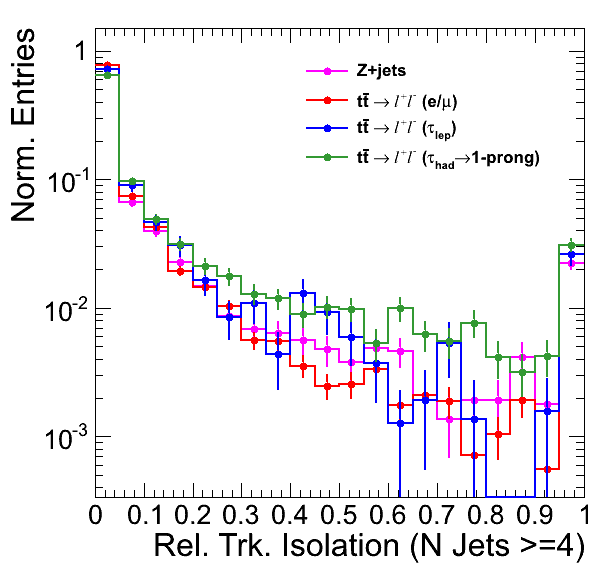
\includegraphics[width=0.5\linewidth]{plots/pfiso_njets4_log.png}%
%	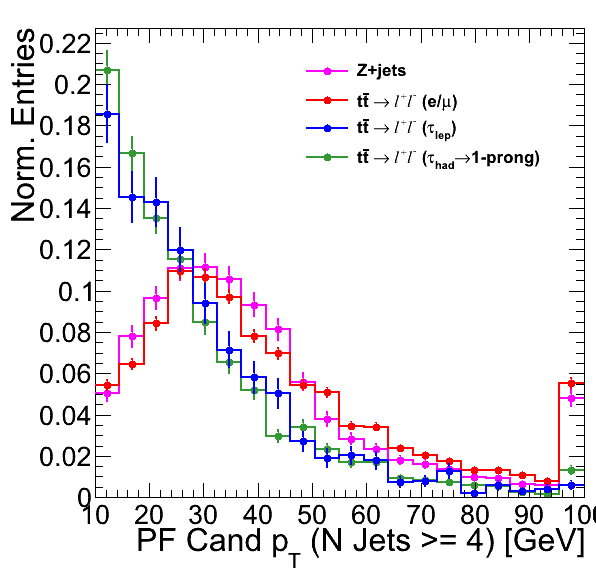
\includegraphics[width=0.5\linewidth]{plots/pfpt_njets4.png}
%	\caption{
%	  \label{fig:reliso}%\protect 
%          Comparison of relative track isolation variable for PF cand probe in Z+jets and ttbar 
%          Z+Jets and ttbar dilepton have similar isolation distributions
%          ttbar with leptonic and single prong taus tend to be less
%          isolated. The difference in the isolation can be attributed
%          to the different \pt\ distribution of the samples, since
%          $\tau$ decay products tend to be softer than leptons arising
%          from \W\ or \Z\ decays.}  
%      \end{center}
%\end{figure}

%	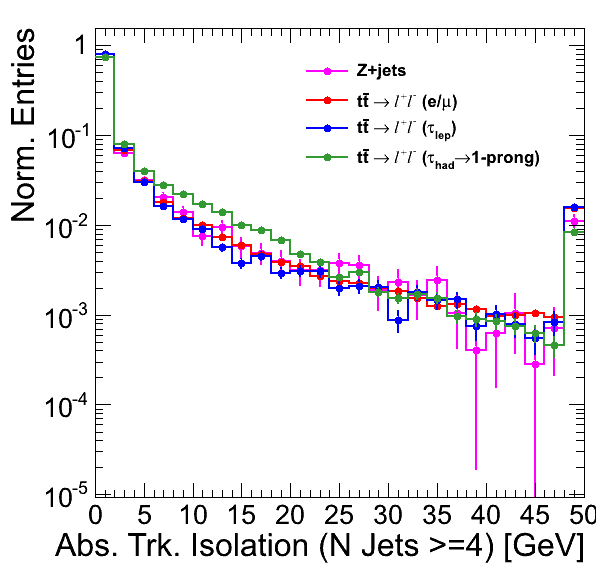
\includegraphics[width=0.5\linewidth]{plots/pfabsiso_njets4_log.png}


%BEGIN SECTION TO WRITE OUT 
%In detail, the procedure to correct the dilepton background is:

%\begin{itemize}
%\item Using tag-and-probe studies, we plot the distribution of {\bf absolute} track isolation for identified probe electrons
%and muons {\bf TODO: need to compare the e vs. $\mu$ track iso distributions, they might differ due to e$\to$e$\gamma$}.
%\item We verify that the distribution of absolute track isolation does not depend on the \pt\ of the probe lepton.
%This is due to the fact that this isolation is from ambient PU and jet activity in the event, which is uncorrelated with
%the lepton \pt {\bf TODO: verify this in data and MC.}.
%\item Our requirement is {\bf relative} track isolation $<$ 0.1. For a given \ttll\ MC event, we determine the \pt of the 2nd
%lepton and translate this to find the corresponding requirement on the {\bf absolute} track isolation, which is simply $0.1\times$\pt.
%\item We measure the efficiency to satisfy this requirement in data and MC, and define a scale-factor $SF_{\epsilon(trk)}$ which
%is the ratio of the data-to-MC efficiencies. This scale-factor is applied to the \ttll\ MC event.
%\item {\bf THING 2 we are unsure about: we can measure this SF for electrons and for muons, but we can't measure it for hadronic 
%tracks from $\tau$ decays. Verena has showed that the absolute track isolation distribution in hadronic $\tau$ tracks is harder due 
%to $\pi^0\to\gamma\gamma$ with $\gamma\to e^+e^-$.}
%\end{itemize} 
%END SECTION TO WRITE OUT 


{\bf fix me: What you have written in the next paragraph does not explain how $\epsilon_{fake}$ is measured.
Why not measure $\epsilon_{fake}$ in the b-veto region?}

%A measurement of the $\epsilon_{fake}$ in data is non-trivial. However, it is
%possible to correct for differences in the $\epsilon_{fake}$ between data and MC by
%applying an additional scale factor for the single lepton background
%alone, using the sample in the \mt\ peak region. This scale factor is determined after applying the isolated track
%veto and after subtracting the \ttll\ component, corrected for the
%isolation efficiency derived previously. 
%As shown in Figure~\ref{fig:vetoeffcomp}, the efficiency for selecting an
%isolated track in single lepton events is independent of \mt\, so the use of
%an overall scale factor is justified to estimate the contribution in
%the \mt\ tail. 
%
%\begin{figure}[hbt]
%  \begin{center}
%	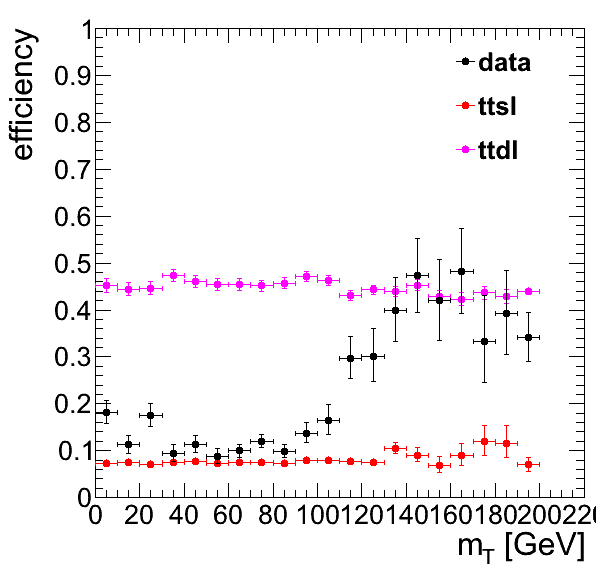
\includegraphics[width=0.5\linewidth]{plots/vetoeff_comp.png}
%	\caption{
%	  \label{fig:vetoeffcomp}%\protect 
%          Efficiency for selecting an isolated track comparing
%          single lepton \ttlj\ and dilepton \ttll\ events in MC and 
%          data as a function of \mt. The
%          efficiencies in \ttlj\ and \ttll\ exhibit no dependence on
%          \mt\, while the data ranges between the two. This behavior
%          is expected since the low \mt\ region is predominantly \ttlj, while the
%          high \mt\ region contains mostly \ttll\ events.}  
%      \end{center}
%\end{figure}

\subsection{Summary of uncertainties}
\label{sec:bgunc-bottomline}.

THIS NEEDS TO BE WRITTEN